\documentclass[%
11pt,%
%oneside,%
twoside,%
%twocolumn,%
titlepage,%
%fleqn,%
%a4page,%
german,%
headsepline%
]{scrartcl}

%\usepackage{fancyhdr}
%\usepackage{scrpage}
\usepackage{lastpage}
\usepackage{geometry}
\usepackage{graphicx}
\usepackage[utf8]{inputenc}
\usepackage[ngerman]{babel}
\usepackage{lscape}
\usepackage[framemethod=TikZ]{mdframed}
\usepackage[most]{tcolorbox}
\usepackage{mymath}
\usepackage{units}
\usepackage{nicefrac}
\usepackage{pgf,tikz,pgfplots}
\pgfplotsset{compat=1.14}
\usepackage{mathrsfs}
\usetikzlibrary{arrows}
\usepackage{colortbl}
\usepackage{hhline}
\usepackage{multirow}
\usepackage[extendedchars]{grffile}
\usepackage{caption}
\usepackage{multicol,calc}
\usepackage{blindtext}
\usepackage{pdfpages}
\usepackage{hyperref}
%\usepackage{tikz-er2}
\usepackage{framed}
\usetikzlibrary{arrows}
\usetikzlibrary{positioning}
\usetikzlibrary{shadows}

\usepackage{marginnote}
\usepackage[]{qrcode}
\qrset{height=9ex}

%\usepackage{romannum}
\usepackage{longtable}
\usepackage{listings}
\usepackage{wrapfig}

\setlength{\parindent}{0cm}


% Command, um Tabellen-Spalten anzupassen
\newcommand{\spaltenheight}{\rule{0mm}{3ex}}
\newcommand{\spaltenwidth}{\rule{3cm}{0mm}}
\newcommand{\spaltensep}{\\[1ex]}
%\arrayrulecolor{darkgreen}
\doublerulesepcolor{white}
\definecolor{lightyellow}{rgb}{1,1,0.8}
\definecolor{Gray}{gray}{0.9}


% Pagestyle/Layout
%\geometry{a4paper , tmargin =2.5cm,	bmargin=3cm, lmargin =2.5cm,	rmargin =2.5cm,	headheight=3em, headsep=1em, footskip=1cm}
%\setlength{\parindent}{0pt} \setlength{\parskip}{1em}
%für TwoSide
%\lhead{\headmark\pagemark}
%\cehead{}
%\rehead{}
%\lohead{}
%\cohead{}
%\rohead{\headmark}
%für OneSide
%\ihead{}
%\chead{}
%\ohead{}
%\setheadsepline{0.5pt} % Linie zur Begrenzung
%\setfootsepline{0.5pt} % Linie zur Begrenzung
\pagestyle{headings} % gemachte Einstellungen anwenden

% Farbig umrahmte Umgebung Satz
 
 \definecolor{myblizzardblue}{HTML}{87CEEB}

\newcounter{satzz}[section]\setcounter{satzz}{0}
\renewcommand{\thesatz}{\arabic{section}.\arabic{satzz}}

\newenvironment{csatz}[2][]{%
    \refstepcounter{satzz}
 
    \ifstrempty{#1}%
    % if condition (without title)
    {\mdfsetup{%
        frametitle={%
            \tikz[baseline=(current bounding box.east),outer sep=0pt]
            \node[anchor=east,rectangle,fill=myblizzardblue]
            {\strut Satz~\thesatz};}
        }%
    % else condition (with title)
    }{\mdfsetup{%
        frametitle={%
            \tikz[baseline=(current bounding box.east),outer sep=0pt]
            \node[anchor=east,rectangle,fill=myblizzardblue]
            {\strut Satz~\thesatz:~#1};}%
        }%
    }%
% for both conditions
    \mdfsetup{%
        innertopmargin=10pt,linecolor=myblizzardblue,%
        backgroundcolor=whitesmoke,%
        linewidth=2pt,topline=true,%
        frametitleaboveskip=\dimexpr-\ht\strutbox\relax%
    }
 
\begin{mdframed}[]\relax}{%
\end{mdframed}}

% Farbig umrahmte Umgebung Theorem
 
\definecolor{mygraphblue}{HTML}{84B7E1}
\definecolor{whitesmoke}{HTML}{F5F5F5}

\newcounter{theo}[section]\setcounter{theo}{0}
\renewcommand{\thetheo}{\arabic{section}.\arabic{theo}}

\newenvironment{ctheo}[2][]{%
    \refstepcounter{theo}
 
    \ifstrempty{#1}%
    % if condition (without title)
    {\mdfsetup{%
        frametitle={%
            \tikz[baseline=(current bounding box.east),outer sep=0pt]
            \node[anchor=east,rectangle,fill=mygraphblue]
            {\strut Theorem~\thetheo};}
        }%
    % else condition (with title)
    }{\mdfsetup{%
        frametitle={%
            \tikz[baseline=(current bounding box.east),outer sep=0pt]
            \node[anchor=east,rectangle,fill=mygraphblue]
            {\strut Theorem~\thetheo:~#1};}%
        }%
    }%
% for both conditions
    \mdfsetup{%
        innertopmargin=10pt,linecolor=mygraphblue,%
        backgroundcolor=whitesmoke,%
        linewidth=2pt,topline=true,%
        frametitleaboveskip=\dimexpr-\ht\strutbox\relax%
    }
 
\begin{mdframed}[]\relax}{%
\end{mdframed}}

% Farbig umrahmte Umgebung Definition
 
 \definecolor{emerald}{HTML}{50C878}

\newcounter{deff}[section]\setcounter{deff}{0}
\renewcommand{\thedeff}{\arabic{section}.\arabic{deff}}

\newenvironment{cdef}[2][]{%
    \refstepcounter{deff}
 
    \ifstrempty{#1}%
    % if condition (without title)
    {\mdfsetup{%
        frametitle={%
            \tikz[baseline=(current bounding box.east),outer sep=0pt]
            \node[anchor=east,rectangle,fill=emerald]
            {\strut Definition~\thedeff};}
        }%
    % else condition (with title)
    }{\mdfsetup{%
        frametitle={%
            \tikz[baseline=(current bounding box.east),outer sep=0pt]
            \node[anchor=east,rectangle,fill=emerald]
            {\strut Definition~\thedeff:~#1};}%
        }%
    }%
% for both conditions
    \mdfsetup{%
        innertopmargin=10pt,linecolor=emerald,%
        backgroundcolor=whitesmoke,%
        linewidth=2pt,topline=true,%
        frametitleaboveskip=\dimexpr-\ht\strutbox\relax%
    }
 
\begin{mdframed}[]\relax}{%
\end{mdframed}}

% Farbig umrahmte Umgebung Achtung
 
 \definecolor{mygraphred}{HTML}{E26A6A}

\newcounter{merkee}[section]\setcounter{merkee}{0}
\renewcommand{\themerkee}{\arabic{section}.\arabic{merkee}}

\newenvironment{cachtung}[2][]{%
    \refstepcounter{merkee}
 
    \ifstrempty{#1}%
    % if condition (without title)
    {\mdfsetup{%
        frametitle={%
            \tikz[baseline=(current bounding box.east),outer sep=0pt]
            \node[anchor=east,rectangle,fill=mygraphred]
            {\strut Achtung};}
        }%
    % else condition (with title)
    }{\mdfsetup{%
        frametitle={%
            \tikz[baseline=(current bounding box.east),outer sep=0pt]
            \node[anchor=east,rectangle,fill=mygraphred]
            {\strut Achtung:~#1};}%
        }%
    }%
% for both conditions
    \mdfsetup{%
        innertopmargin=10pt,linecolor=mygraphred,%
        backgroundcolor=whitesmoke,%
        linewidth=2pt,topline=true,%
        frametitleaboveskip=\dimexpr-\ht\strutbox\relax%
    }
 
\begin{mdframed}[]\relax}{%
\end{mdframed}}

\subject{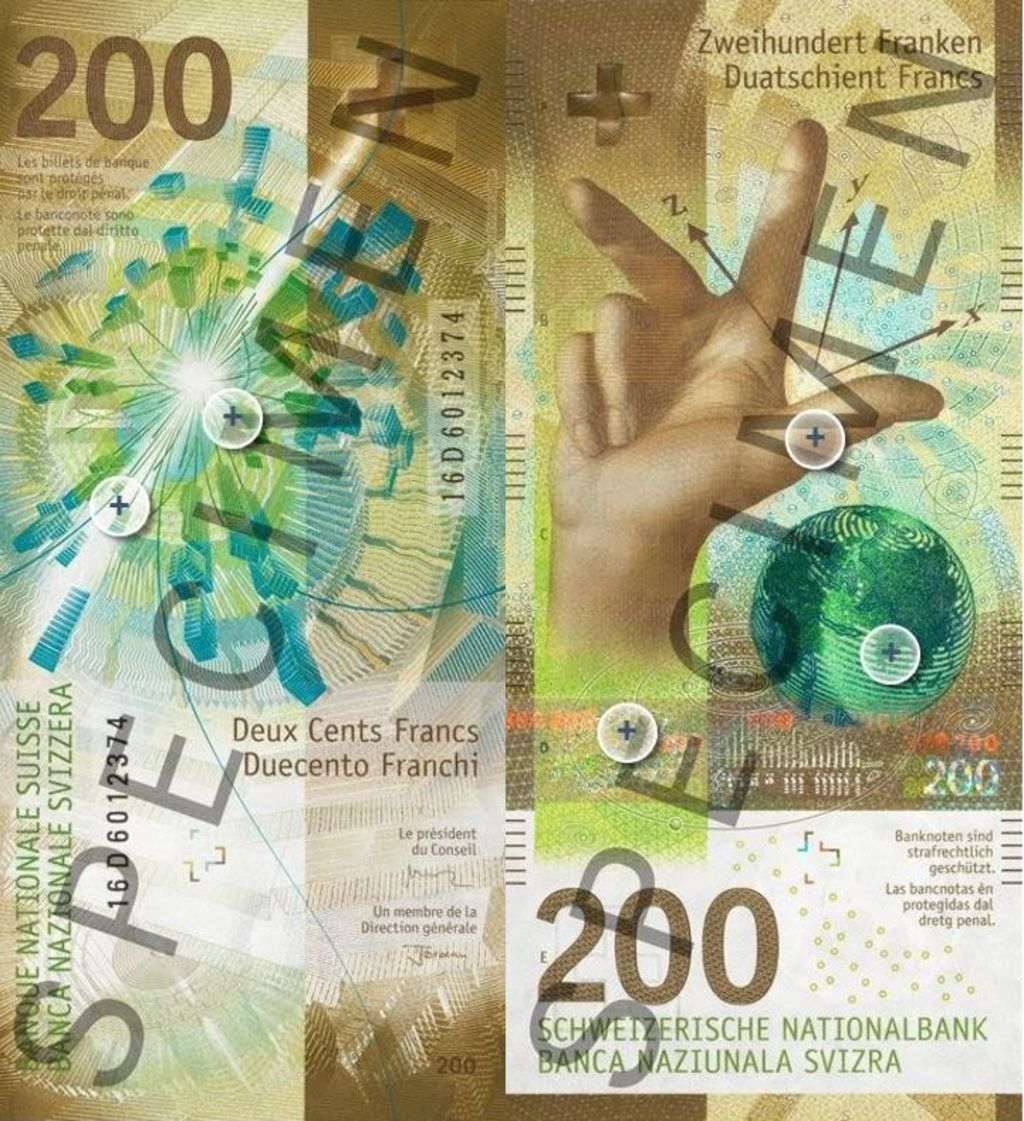
\includegraphics[width=0.618\textwidth]{pictures/200er}}
\title{Vektoren}
\subtitle{Raus in den 3D}
\author{}
\date{}
%\lowertitleback{
%\includegraphics[height=1.1cm]{/Users/jormawassmer/Pictures/logokoeniz.jpg}%
%\copyright Jorma Wassmer
%1. Auflage, Februar 2011
%}


\begin{document}
\maketitle
\tableofcontents
%\thispagestyle{empty}
\cleardoublepage
%\setcounter{page}{1}

\section{Grundbegriffe}

Wenn man die Entwicklung der Mathematik betrachtet, so erkennt man, dass immer wieder neue Begriffe eingeführt werden mussten, weil die vorher verwendeten Begriffe für neue Probleme nicht mehr ausreichten. Oft wurden die Begriffe auch so gewählt, dass sich mit ihnen die bisherigen Probleme leichter bewältigen liessen. Ein typisches Beispiel dafür ist der Begriff des Vektors. Wer sich bereits etwas mit Vektoren auskennt, für den sei hier am Rande der QR-Code zum Video \emph{Vektoren in 10 Minuten} angedacht.
\marginnote{
\qrcode{
https://www.youtube.com/watch?v=tw6_eu___Sk}
}

In unserer Umwelt werden viele Grössen durch Angabe einer reellen Zahl und einer bestimmten Masseinheit beschrieben, z.B. $\unit[10]{s}$, $\unit[4.5]{m^3}$, $\unit[-5]{^\circ C}$, $\unit[100]{g}$. Diese Grössen lassen sich jeweils auf einer Skala (von scalae, lat., Leiter), also durch Punkte auf einer Zahlengeraden, darstellen und heissen deshalb skalare Grössen.

\begin{cdef}[Skalar]{}
Ein \textbf{Skalar} ist eine reelle Zahl.
\end{cdef}

Die Geschwindigkeit hingegen ist ein Beispiel für eine Grösse, zu deren vollständiger Festlegung ausser einer Zahl noch die Angabe einer Richtung nötig ist. Die Existenz und Unabhängigkeit dieser beiden Elemente bei der Festsetzung lassen sich am Beispiel eines Schiffskapitäns, der mit verschiedenen seiner Untergebenen in Verbindung steht, erläutern: Er gibt dem ersten Maschinisten die Knotenzahl (z.B. $\unit[30]{Kn} = \unitfrac[30]{sm}{h}$ oder volle Kraft) bekannt, mit der er fahren, und dem Steuermann die Richtung (z.B. $5$ Grad Backbord), welche er einhalten soll.

Auch eine Kraft wird erst durch Angabe von Betrag, Richtung und An\-griffs\-punkt voll\-ständig beschrieben.

Derartige Grössen, also Grössen, die durch Festlegung eines Betrags und einer Richtung vollständig bestimmt sind, werden vektorielle Grössen genannt und durch Pfeile (gerichtete Strecken) dargestellt.

Mathematisch werden sie durch Vektoren (vehere, lat., fahren) beschrieben. Man definiert:
\begin{cdef}[Vektor]{}
Unter einem \textbf{Vektor}
\marginnote{
\qrcode{
https://m.youtube.com/watch?v=WQ2C4uj5QzA}
}
versteht man eine Schar aus sämtlichen untereinander parallelen, gleichgerichteten und gleichlangen Strecken.
\end{cdef}

\begin{figure}[ht]
\begin{center}
\begin{tikzpicture}[line cap=round,line join=round,>=triangle 45,x=0.4cm,y=0.3cm]
\clip(-4.3,-3.12) rectangle (13.86,6.3);
\draw [->] (-2,1) -- (0,4);
\draw [->] (-1,-1) -- (1,2);
\draw [->] (5,3) -- (7,6);
\draw [->] (7,-2) -- (9,1);
\draw [->] (8,1) -- (10,4);
\draw [->] (10,-1) -- (12,2);
\draw [->] (2,-2) -- (4,1);
\end{tikzpicture}
\end{center}
\caption{Vektor-Schar}
\end{figure}

Damit ist ein Vektor eine unendliche Menge von gerichteten Strecken: Von jedem Punkt der Ebene bzw. des Raumes geht genau eine solche Strecke aus, wobei alle diese Strecken untereinander parallel und gleichgerichtet sind und die gleiche Länge haben.

In Abbildungen wird ein Vektor als eine Strecke mit Pfeilspitze gezeichnet, d.h. man zeichnet nicht die ganze Schar von gerichteten Strecken, die den Vektor darstellen, sondern nur eine dieser Strecken, einen sogenannten \glqq \textbf{Repräsentanten}\grqq.

\begin{figure}
\begin{center}
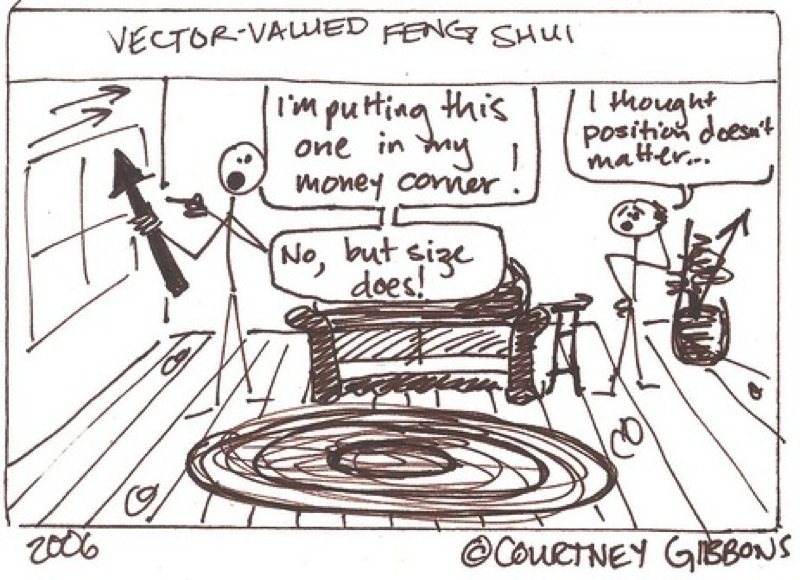
\includegraphics[width=0.618\textwidth]{pictures/repraesentant}
\end{center}
\caption{Repräsentant}
\end{figure}

\begin{bem}
Eine ähnliche Situation liegt bei den Zahlen vor: Vergleiche die Brüche
$$\frac{1}{4}, \frac{2}{8}, \frac{-3}{-12}, \frac{90}{360}, \dots$$
die durch Kürzen und Erweitern auseinander hervorgehen. Sie sind alle dem gleichen Punkt auf der Zahlengeraden zugeordnet. Jeder derartige Bruch kann als Repräsentant zur Angabe der rationalen Zahl $0.25$ herangezogen werden.
\end{bem}

Die Vektoren werden mit $\va, \vb, \V{c}, \vv, \vw, \dots$ oder mit $\V{AB}, \V{PQ},\dots$ (wobei der erste Buchstabe den Anfangspunkt, der zweite den Endpunkt angibt), bezeichnet.
Der darüber gesetzte Pfeil deutet an, dass es sich um einen Vektor und nicht etwa \glqq nur\grqq\ um eine Strecke handelt.

Die \emph{Länge} (der Betrag) eines Vektors schreibt man in der Form $\abs{\vv}$ (oder auch kurz als $v$) bzw. $\abs{\V{PQ}}$; für die Richtung verwendet man kein besonderes Zeichen. Man gibt zum Beispiel in der Ebene die \emph{Richtung} als Winkel zwischen Vektor und positiver $x$-Achse an.

\begin{figure}[ht]
\begin{center}
\definecolor{qqwuqq}{rgb}{0,0.39,0}
\definecolor{cqcqcq}{rgb}{0.75,0.75,0.75}
\scalebox{1.2}{
\begin{tikzpicture}[line cap=round,line join=round,>=triangle 45,x=0.5cm,y=0.5cm]
\draw [color=cqcqcq,dash pattern=on 2pt off 2pt, xstep=0.5cm,ystep=0.5cm] (-3.5,-2.6) grid (6.8,3.5);
\draw[->,color=black] (-4.04,0) -- (7.94,0);
\foreach \x in {-4,-3,-2,-1,1,2,3,4,5,6,7}
\draw[shift={(\x,0)},color=black] (0pt,2pt) -- (0pt,-2pt) node[below] {\footnotesize $\x$};
\draw[color=black] (7.6,0.08) node [anchor=south west] {$x$};
\draw[->,color=black] (0,-2.98) -- (0,4.34);
\foreach \y in {-2,-1,1,2,3,4}
\draw[shift={(0,\y)},color=black] (2pt,0pt) -- (-2pt,0pt) node[left] {\footnotesize $\y$};
\draw[color=black] (0.1,3.94) node [anchor=west] {$y$};
\draw[color=black] (0pt,-10pt) node[right] {\footnotesize $0$};
\clip(-4.04,-2.98) rectangle (7.94,4.34);
\draw [shift={(5,1)},color=qqwuqq,fill=qqwuqq,fill opacity=0.05] (0,0) -- (0:1) arc (0:153.43:1) -- cycle;
\draw [->] (5,1) -- (1,3);
\draw[color=black] (3.14,2.4) node {$\vv$};
\draw[color=qqwuqq] (5.1,1.4) node {$\varphi$};
\end{tikzpicture}
}
\end{center}
\caption{Betrag und Richtung}\label{vecdef}
\end{figure}

\begin{ueb}[Länge und Richtung]
Bestimme Länge und Richtung von $\vv$ aus Abbildung \ref{vecdef} auf Seite \pageref{vecdef}.
\end{ueb}

Mit der blossen Definition von Vektoren hat man natürlich noch nicht viel erreicht. Entscheidend für die Einführung von Vektoren ist die Tatsache, dass man für sie Rechengesetze angeben und infolgedessen mit ihnen --- ähnlich wie in der Arithmetik mit Zahlen oder in der Algebra mit Buchstaben --- rechnen kann. Dies wird das Ziel der folgenden Kapitel sein.

\begin{bem}
Um die algebraische Struktur, auf denen die einzuführenden Rechengesetze gelten, zu vervollständigen, lässt man Strecken der Länge Null zu, also Punkte. Obwohl für solche Strecken keine Richtung definiert ist, ist es zweckmässig, diese als Nullvektor $\V{0}$ zu bezeichnen. Der Nullvektor hat den Betrag $0$ und keine Richtung.
\end{bem}

Oft ist es beim Rechnen mit Vektoren hilfreich, die Aufgabenstellung geometrisch zu interpretieren. So wie die Spiegelungen durch ein einziges geometrisches Objekt festgelegt werden --- nämlich durch ein Symmetriezentrum, eine Symmetrieachse oder eine Symmetrieebene --- wird auch die Translation durch ein einziges geometrisches Objekt festgelegt, nämlich durch einen Vektor $\vv$.
\begin{bem}
Ein Vektor kann geometrisch als Translation aufgefasst werden, der den Anfangspunkt in den Endpunkt abbildet.
\end{bem}

Die Grundlagen zur heutigen Vektorrechnung legten erst in der Mitte des 19. Jahrhunderts fast gleichzeitig und doch völlig unabhängig voneinander der Schotte \textsc{Sir William Rowan Hamilton} (1805- 1865) und der Deutsche \textsc{Hermann Günther Grassmann} (1809-1877). \textsc{Hamilton} war ein eigenwilliges Genie, konnte bereits mit zehn Jahren \textsc{Homer} auswendig und erlernte in den nächsten Jahren dreizehn Sprachen. 1827 wurde er Professor der Astronomie an der Universität von Dublin, wo er bis zu seinem Tode blieb. 1845 führte er in einer Abhandlung den Begriff des Vektors erstmalig ein und baute ihn in seinen Werken über \glqq Quaternionen\grqq\ weiter aus. \textsc{Grassmann} war Gymnasiallehrer für Mathematik in Stettin. Sein erstes Werk erschien 1844, wurde aber fast 18 Jahre lang nicht beachtet. Erst sein zweites Werk von 1862 brachte ihm den verdienten Durchbruch.

Heute gilt die Vektorrechnung in der Mathematik und ihren Anwendungen in den Naturwissenschaften als ein unentbehrliches Hilfsmittel. Als herausragendes Beispiel seien hier nur die vier Maxwell'schen Vektorgleichungen erwähnt, die für die Elektrodynamik ein ähnliches Axiomensystem wie die Newton'schen Grundgleichungen für die Mechanik bilden (\textsc{James Clerk Maxwell}, 1831-1879).

\begin{align*}
\nabla\cdot\V{E} &= \frac{\gr}{\ge_0}\tag{Ladung ist Quelle des elektrischen Feldes}\\
\nabla\cdot\V{B} &= 0\tag{Es gibt keine magnetischen Monopole}\\
\nabla\times\V{E} &= -\frac{\partial \V{B}}{\partial t}\tag{\"Anderung mag. Feld führt zu el. Wirbelfeld}\\
\nabla\times\V{B} &= \gm_0\V{j}+\gm_0\epsilon_0\frac{\partial\V{E}}{\partial t}\tag{el. Strom führt zu mag. Wirbelfeld}
\end{align*}

\begin{ueb}[Betrag und Richtung]
Berechne die Beträge und die Richtungen (Winkel $\varphi$ zwischen Pfeil und $x$-Achse) der eingezeichneten Vektoren.
\begin{center}
\definecolor{cqcqcq}{rgb}{0.75,0.75,0.75}
\begin{tikzpicture}[line cap=round,line join=round,>=triangle 45,x=0.45cm,y=0.45cm]
\draw [color=cqcqcq,dash pattern=on 2pt off 2pt, xstep=0.45cm,ystep=0.45cm] (-7.56,-5.2) grid (7.4,4.5);
\draw[->,color=black] (-7.56,0) -- (8.16,0);
\foreach \x in {-7,-6,-5,-4,-3,-2,-1,1,2,3,4,5,6,7,8}
\draw[shift={(\x,0)},color=black] (0pt,2pt) -- (0pt,-2pt) node[below] {\footnotesize $\x$};
\draw[color=black] (7.82,0.08) node [anchor=south west] { x};
\draw[->,color=black] (0,-5.56) -- (0,5.54);
\foreach \y in {-5,-4,-3,-2,-1,1,2,3,4,5}
\draw[shift={(0,\y)},color=black] (2pt,0pt) -- (-2pt,0pt) node[left] {\footnotesize $\y$};
\draw[color=black] (0.1,5.14) node [anchor=west] { y};
\clip(-7.56,-5.56) rectangle (8.16,5.54);
\draw [->] (-1,4) -- (-7,2);
\draw [->] (-5,-4) -- (-3,1);
\draw [->] (1,1) -- (6,2);
\draw [->] (2,-2) -- (4,-2);
\draw [->] (6.5,-5) -- (-2,-3);
\draw[color=black] (-4.1,3.5) node {$\V{u}$};
\draw[color=black] (-4.4,-1.32) node {$\vv$};
\draw[color=black] (3.26,1.9) node {$\vw$};
\draw[color=black] (2.96,-1.4) node {$\vb$};
\draw[color=black] (2.5,-3.5) node {$\va$};
\end{tikzpicture}
\end{center}
\end{ueb}

\section{Grundoperationen mit Vektoren}
Wir wollen uns zuerst mit der geometrischen Interpretation der Grundoperationen auseinandersetzen. Die algebraische Umsetzung ist dann \glqq einfach\grqq\ durch Angabe von Definitionen zu erledigen, die die Geometrie repräsentieren.
\subsection{Gegenvektor}
\begin{cdef}[Gegenvektor]{}
Der Vektor, der zwar den gleichen Betrag, aber die entgegengesetzte Richtung wie $\vv$ hat, wird mit $-\vv$ bezeichnet und heisst \textbf{Gegenvektor} von $\vv$.
\end{cdef}

\begin{figure}[ht]
\begin{center}
\definecolor{cqcqcq}{rgb}{0.75,0.75,0.75}
\scalebox{1.3}{
\begin{tikzpicture}[line cap=round,line join=round,>=triangle 45,x=0.6cm,y=0.6cm]
\draw [color=cqcqcq,dash pattern=on 3pt off 3pt, xstep=0.3cm,ystep=0.3cm] (-4.3,1.16) grid (6.72,6.3);
\clip(-4.3,1.16) rectangle (6.72,6.3);
\draw [->] (3,5) -- (-3,3);
\draw [->] (-1,2) -- (5,4);
\end{tikzpicture}
}
\end{center}
\caption{Vektor und Gegenvektor}
\end{figure}

\subsection{S-Multiplikation}
Analog definiert man die Multiplikation eines Vektors mit einem Skalar.
\begin{cdef}[S-Multiplikation]{}
Für $t\in\mR$ ist $t\cdot\va$ ein Vektor mit dem $\abs{t}$-fachen Betrag von $\va$:
$$\abs{t\va}=\abs{t}\va.$$
Diese Operation nennt man kurz \textbf{S-Multiplikation}.
\begin{itemize}
\item Falls $t>0$ ist, hat $t\va$ dieselbe Richtung wie $\va$,
\item Falls $t<0$ ist, hat $t\va$ die entgegengesetzte Richtung von $\va$,
\item falls $t=0$ ist, ist $t\va$ der Nullvektor.
\end{itemize}
\end{cdef}

\begin{figure}[ht]
\begin{center}
\definecolor{qqqqff}{rgb}{0,0,1}
\begin{tikzpicture}[line cap=round,line join=round,>=triangle 45,x=0.618cm,y=0.618cm]
\clip(-0.18,-1.04) rectangle (8.9,4.24);
\draw [->] (0.5,0.5) -- (1.5,2.5);
\draw [->] (2,-0.5) -- (4,3.5);
\draw [->] (6,3) -- (4.5,0);
\draw[color=black] (0.6,1.5) node {$\vv$};
\draw[color=black] (2.6,1.68) node {$2\vv$};
\draw[color=black] (4.3,1.5) node {$-1.5\vv$};
\fill [color=qqqqff] (7.5,1.5) circle (1.5pt);
\draw[color=black] (7.66,1.9) node {$\V{0}$};
\end{tikzpicture}
\end{center}
\caption{S-Multiplikation}
\end{figure}

Umgekehrt gilt
\begin{csatz}[Satz zur Parallelität]{}
Sind zwei Vektoren $\vv$ und $\vw$ zu ein und derselben Geraden parallel, so ist $\vw$ ein Vielfaches von $\vv$, d.h.
$$\vw=t\vv$$
\end{csatz}

\begin{proof}
trivial
\end{proof}

\begin{cdef}[kollinear]{}
Zwei Vektoren $\vv$ und $\vw$, für die $$\vw=t\vv$$ gilt, heissen \textbf{kollinear}.
\end{cdef}

\begin{cdef}[Einheitsvektor]{}
Ein Vektor mit Betrag $1$ heisst \textbf{Einheitsvektor}.
\end{cdef}

\subsection{Addition und Subtraktion}
Man legt fest
\begin{cdef}[Addition]{}
Die \textbf{Summe}
\marginnote{
\qrcode{
https://m.youtube.com/watch?v=eiIF6NDyYqU}
}
$\vv+\vw$ zweier Vektoren $\vv$ und $\vw$ ist der Vektor $\V{u}$, den man durch \glqq Aneinandersetzen\grqq\ von $\vv$ und $\vw$ erhält.
\end{cdef}

\begin{figure}[ht]
\begin{center}
\definecolor{qqqqff}{rgb}{0,0,1}
\begin{tikzpicture}[line cap=round,line join=round,>=triangle 45,x=0.5cm,y=0.4cm]
\clip(-4.3,-1.26) rectangle (7.06,6.3);
\draw [->] (-3,0) -- (3,0);
\draw [->] (3,0) -- (6,5);
\draw [->,dash pattern=on 2pt off 2pt] (-3,0) -- (6,5);
\fill [color=qqqqff] (-3,0) circle (1.5pt);
\draw[color=qqqqff] (-3.5,0.18) node {$A$};
\fill [color=qqqqff] (3,0) circle (1.5pt);
\draw[color=qqqqff] (3.4,-0.08) node {$B$};
\draw[color=black] (-0.02,-0.4) node {$\vv$};
\fill [color=qqqqff] (6,5) circle (1.5pt);
\draw[color=qqqqff] (6.16,5.5) node {$C$};
\draw[color=black] (4.9,2.32) node {$\vw$};
\draw[color=black] (0.2,3.1) node {$\vu=\vv+\vw$};
\end{tikzpicture}
\end{center}
\caption{Vektoraddition}
\end{figure}

Der Summenvektor $\vu=\vv+\vw$ hat seinen Anfangspunkt im Anfangspunkt des ersten Summanden und seinen Endpunkt im Endpunkt des zweiten Summanden:
$$\V{AB}+\V{BC}=\V{AC}$$

\begin{bem}
$\vu=\vv+\vw$ entspricht der Diagonalen des von $\vv$ und $\vw$ aufgespannten Parallelogramms.
\end{bem}

\begin{bem}
Mit dieser Definition erzielt man auch eine Übereinstimmung mit dem in der Physik experimentell nachgewiesenen \glqq Kräfteparallelogramm\grqq. Wenn an einem Körper die Kräfte $\V{F_1}$ und $\V{F_2}$ am gleichen Punkt angreifen, dann können sie durch die \emph{resultierende} Kraft $\V{F_R}$ ersetzt werden, welche die \emph{vektorielle} Summe der angreifenden Kräfte ist:
$$\V{F_R} = \V{F_1} + \V{F_2}$$

\begin{figure}[ht]
\begin{center}
\definecolor{cqcqcq}{rgb}{0.75,0.75,0.75}
\scalebox{0.8}{
\begin{tikzpicture}[line cap=round,line join=round,>=triangle 45,x=0.7cm,y=0.8cm]
\clip(-4.26,-1.3) rectangle (5.58,4.52);
\draw [->] (-3,0) -- (3,0);
\draw [->] (-3,0) -- (-1,4);
\draw [dash pattern=on 5pt off 5pt] (-1,4)-- (5,4);
\draw [dash pattern=on 5pt off 5pt] (5,4)-- (3,0);
\draw [->] (-3,0) -- (5,4);
\draw [rotate around={-64.87:(-2.92,0.09)},fill=black,fill opacity=0.15] (-2.92,0.09) ellipse (1.15cm and 0.73cm);
\draw[color=black] (0.04,-0.26) node {$\V{F_1}$};
\draw[color=black] (-2.3,2.38) node {$\V{F_2}$};
\draw[color=black] (1,2.5) node {$\V{F_R}$};
\end{tikzpicture}
}
\end{center}
\caption{Kräfteparallelogramm}
\end{figure}
\end{bem}

\begin{cdef}[Subtraktion]{}
Die \textbf{Subtraktion} wird auf die Addition zurückgeführt:
$$\vu=\vv-\vw=\vv+(-\vw)$$
\end{cdef}
Man subtrahiert den Vektor $\vw$ vom Vektor $\vv$, indem
man zu $\vv$ den Gegenvektor von $\vw$ addiert. Aus $\vu=\vv-\vw$ ergibt sich sofort $\vu+\vw=\vv$. Um die Differenz $\vv-\vw$ zu erhalten, genügt es, die Vektoren $\vv$ und $\vw$ an einem Punkt $P$ anzutragen und den Vektor aufzusuchen, der vom Endpunkt des Vektors $\vw$ zum Endpunkt des Vektors $\vv$ reicht.

\begin{figure}[ht]
\begin{center}
\begin{tikzpicture}[line cap=round,line join=round,>=triangle 45,x=0.8cm,y=0.8cm]
\clip(-4.26,-0.76) rectangle (3.7,4.52);
\draw [->] (-3,1.5) -- (-2,3.5);
\draw [->] (-4,0.5) -- (-1,0.02);
\draw [->] (0,1) -- (1,3);
\draw [->] (0,1) -- (3,0.5);
\draw [->] (3,0.5) -- (1,3);
\draw[color=black] (-2.82,2.66) node {$\vv$};
\draw[color=black] (-2.58,0.62) node {$\vw$};
\draw[color=black] (0.2,2.04) node {$\vv$};
\draw[color=black] (1.26,0.58) node {$\vw$};
\draw[color=black] (2.14,2.06) node {$\vu$};
\end{tikzpicture}
\end{center}
\caption{Subtraktion von Vektoren}
\end{figure}

Die folgenden Rechenregeln für die Vektoraddition und die S-Multiplikation lassen sich unmittelbar ableiten. Für $\vu,\vv,\vw\in\mR^3$ und $\gl, \gm\in\mR$ gilt:
\begin{itemize}
\item Kommutativität: $$\vv+\vw=\vw+\vv$$
\item Assoziativität: $$\vu+(\vv+\vw)=(\vu+\vv)+\vw$$
\item Neutrales Element: $$\vv+\V{0}=\vv$$
\item Inverse Elemente: $$\vv+(-\vv)=\V{0}$$
\item Ausklammerungsregel: $$\gl(\vv+\vw)=\gl\vv+\gl\vw$$
\item S-Faktorisierung: $$(\gl+\gm)\vv=\gl\vv+\gm\vv$$
\item Gemischte Assoziativität: $$\gl(\gm\vv)=(\gl\gm)\vv$$
\end{itemize}
Diese Regeln, die wir hier nicht einzeln beweisen, erlauben uns, mit Vektoren genau so zu rechnen, wie wir es von der Algebra her gewohnt sind.

\begin{ueb}[Pfeilchen zeichnen]
Gegeben seien die Vektoren $\vu,\vv$ und $\vw$.

\begin{center}
\definecolor{cqcqcq}{rgb}{0.75,0.75,0.75}
\begin{tikzpicture}[line cap=round,line join=round,>=triangle 45,x=0.9cm,y=0.9cm]
\draw [color=cqcqcq,dash pattern=on 2pt off 2pt, xstep=0.5cm,ystep=0.5cm] (-4.26,0.16) grid (2.4,4.4);
\clip(-4.26,0.16) rectangle (2.58,4.52);
\draw [->] (-3.5,4) -- (-1.5,3);
\draw [->] (-4,1.5) -- (-1,1.5);
\draw [->] (0,1) -- (2,3);
\draw[color=black] (-2.42,3.72) node {$\vu$};
\draw[color=black] (-2.44,1.72) node {$\vv$};
\draw[color=black] (0.72,2.24) node {$\vw$};
\end{tikzpicture}
\end{center}
Skizziere:
\begin{enumeratea}
\item $\vr=\vu-\vv$
\item $\va=\vu-2\vv+0.5\vw$
\item $\vb=3\vu+1.5\vv-4\vw$
\item $\vc$ so, dass $\vu-2\vv+\vc=\vw$ gilt.
\end{enumeratea}
\end{ueb}

\begin{ueb}[Ab in die Aare!]
Ein
\marginnote{
\qrcode{
https://m.youtube.com/watch?v=yrQB3sX_HOM}
}
Schwimmer ($v_s = \unitfrac[1.5]{m}{s}$) will einen $\unit[20]{m}$ breiten Fluss ($v_F = \unitfrac[1.2]{m}{s}$)
\begin{enumeratea}
\item auf kürzestem Wege,
\item in kürzester Zeit
\end{enumeratea}
überqueren. Berechne jeweils die Dauer und zusätzlich
\begin{enumeratea}
\item den Vorhaltewinkel
\item die Abdrift.
\end{enumeratea}
\end{ueb}

\begin{ueb}[Beweis Mittellinie]
Zeige, dass die Mittellinie eines Dreiecks halb so
lang wie die Grundlinie und parallel zu dieser ist.
\end{ueb}

\begin{ueb}[Beweis halbierte Diagonalen]
Halbieren
\marginnote{
\qrcode{
https://m.youtube.com/watch?v=mbfcd-n5saI}
}
sich in einem Viereck die Diagonalen, so ist es ein Parallelogramm?!
\end{ueb}

Ein ausserordentlich nützlicher Satz lässt sich über nicht kollineare Vektoren formulieren:
\begin{csatz}[Satz zur linearen Abhängigkeit]{}\label{csatzlinunabh}
Sind $\vv$ und $\vw$ nicht kollinear und $$\gl\vv+\gm\vw=\V{0},$$ dann muss $\gl=0$ \emph{und} $\gm=0$ sein.
\end{csatz}
\begin{proof}[Beweis]
Es seien $\vv$ und $\vw$ nicht kollinear abhängig und $\gl\vv+\gm\vw=\V{0}$. OEdA $\gl\neq0$, dann gälte $\vv=-\frac{\gm}{\gl}\vw$. Dies ist ein Widerspruch zur Annahme, dass $\vv$ und $\vw$ nicht kollinear sind. Analog geht man für $\gm$ vor.
\end{proof}
Die lineare Unabhängigkeit zweier Vektoren $\vv$ und $\vw$ lässt sich geometrisch veranschaulichen, wenn man die Diagonale des von $\gl\vv$ und $\gm\vw$ aufgespannten Parallelogramms betrachtet. Diese Diagonale entspricht nur dann dem Nullvektor, wenn $\gl=0$ und zugleich $\gm=0$ wird.

\begin{cdef}[lineare Unabhängigkeit]{}
Man nennt zwei nicht kollineare Vektoren \textbf{linear unabhängig}.
\end{cdef}

\begin{bem}
Mit Satz \ref{csatzlinunabh} lassen sich sehr elegant bekannte Sätze aus der Elementargeometrie beweisen.
\end{bem}

\begin{ueb}[Parallelogramm-Eigenschaft]
Zeige, dass sich in einem Parallelogramm die Diagonalen halbieren.
\end{ueb}

\section{Vektoren im Koordinatensystem}
Wir wollen in diesem Kapitel zunächst nur ein rechtwinkliges Koordinatensystem zugrundelegen; am Ende des Kapitels soll dann --- für Interessierte --- kurz auf affine Koordinatensysteme eingegangen werden.
Durch Parallelverschiebung kann man \glqq Pfeile\grqq, die ja Vektoren repräsentieren, so verschieben, dass ihre Anfangspunkte auf den Ursprung $0$ eines rechtwinkligen Koordinatensystems zu liegen kommen. Diese an einen festen Ort gebundenen Repräsentanten nennt man \textbf{Ortsvektoren}.

Die Einheitsvektoren $\ex$ und $\ey$ in Richtung der $x$-Achse bzw. $y$-Achse werden Basisvektoren genannt; denn sie bilden eine Basis und erlauben uns, einen beliebigen Ortsvektor $\vv$ der $xy$-Ebene zu \glqq zerlegen\grqq.
\begin{figure}[ht]
\begin{center}
\begin{tikzpicture}[line cap=round,line join=round,>=triangle 45,x=0.69cm,y=0.69cm]
\draw[->,color=black] (-1.1,0) -- (8,0);
\foreach \x in {2,4,6}
\draw[shift={(\x,0)},color=black] (0pt,2pt) -- (0pt,-2pt);
\draw[color=black] (7.66,0.08) node [anchor=south west] { x};
\draw[->,color=black] (0,-1.14) -- (0,5.16);
\foreach \y in {2,4}
\draw[shift={(0,\y)},color=black] (2pt,0pt) -- (-2pt,0pt);
\draw[color=black] (0.1,4.76) node [anchor=west] { y};
\clip(-1.1,-1.14) rectangle (8,5.16);
\draw [->] (0,0) -- (0,2);
\draw [->] (0,0) -- (2,0);
\draw [->] (0,0) -- (5.5,4);
\draw [->] (0,0) -- (5.42,0);
\draw [->] (5.42,0) -- (5.5,4);
\draw[color=black] (-0.4,1.06) node {$\ey$};
\draw[color=black] (0.86,-0.4) node {$\ex$};
\draw[color=black] (2.6,2.5) node {$\vv$};
\draw[color=black] (3.1,-0.4) node {$\gl\ex$};
\draw[color=black] (6,2.1) node {$\gm\ey$};
\end{tikzpicture}
\end{center}
\caption{Zerlegung in Basisvektoren: $\vv=\gl\ex+\gm\ey$}
\end{figure}
Die Vektoren $\gl\ex$ und $\gm\ey$ der Zerlegung von $\vv$ nennt man die vektoriellen Komponenten von $\vv$ bezüglich der Basis $\set{\ex,\ey}$.
Die Koeffizienten $\gl$ und $\gm$ in der Zerlegung des Vektors
$$\vv=\gl\ex+\gm\ey$$
nennt man die skalaren Komponenten, oder einfacher, die \textbf{Koordinaten} des Vektors $\vv$ bezüglich der Basis $\set{\ex,\ey}$.

\begin{bem}
Will man Punkt\-koordi\-naten und Vektor\-koordi\-naten voneinander unterscheiden, so kann man Punkt\-koordi\-naten nebeneinander, zum Beispiel $P\point{-3}{4}$, und  Vektor\-koordi\-naten untereinander schreiben; exemplarisch
$$\vv=\begin{pmatrix}3\\7\end{pmatrix}.$$

Theoretisch ist es aber nicht nötig, Punkt und Vektor zu unterscheiden. Wir identifizieren einen Punkt einfach mit dem entsprechenden Ortsvektor. Aus dem Kontext geht jeweils klar hervor, ob man mit Punkten oder Vektoren arbeitet. Ich werde beide Schreibweisen je nach Praktikabilität anwenden.
\end{bem}

\begin{cdef}[Vektorschreibweise]{}
Statt $\vv= x\cdot\ex+y\cdot\ey$ schreibt man kürzer:
$$\begin{pmatrix}x\\y\end{pmatrix}$$
\end{cdef}

\begin{csatz}[Länge]{}
Für die Länge von $\vv=\point{x}{y}$ gilt
$$v=\sqrt{x^2+y^2}.$$
\end{csatz}
\begin{proof}[Beweis]
Der Satz folgt direkt aus Pythagoras und $\abs{\ex}=\abs{\ey}=1$.
\end{proof}

\section{Anwendungen}
\subsection{Impuls}
Multipliziert man die skalare Grösse $m$ (Masse) mit der vektoriellen Grösse $\vv$ (Geschwindigkeit), so erhält man mit dieser S-Multiplikation den Impuls $\V{p}$.

Der Impuls ist eine vektorielle Grösse mit der Richtung der Geschwindigkeit:
$$\V{p}=m\cdot\vv.$$

\begin{csatz}[Impulserhaltung]{}
Die vektorielle Summe der Impulse eines abgeschlossenen Systems ist zeitlich konstant.
\end{csatz}
Anders ausgedrückt: Die Summe der Impulse vor einer Kollision ist gleich der Summe der Impulse nach der Kollision.

\begin{ueb}[Lastwagen]
Ein $\unit[6]{t}$ schwerer Lastwagen, der mit $\unitfrac[15]{km}{h}$ in Richtung Norden fährt, kollidiert mit einem $\unit[4]{t}$ schweren Lastwagen, der mit $\unitfrac[45]{km}{h}$ in Richtung Westen fährt. Mit welcher Geschwindigkeit und in welcher Richtung bewegen sich die beiden Lastwagen nach der Kollision, wenn sie miteinander verbunden bleiben?
\end{ueb}

\begin{ueb}[Stern]
Ein Stern mit der Masse $m_1 = \unit[2\cdot10^{30}]{kg}$ bewegt sich mit der Geschwindigkeit $\V{v_1}=\unitfrac[2\cdot10^4]{m}{s}$. Dabei kollidiert er mit einem zweiten Stern ($m_2 = \unit[5\cdot10^{30}]{kg}$, $\V{v_2} = \unitfrac[3\cdot10^4]{m}{s}$). Ihre Bahnen bilden einen rechten Winkel. Nach der Kollision bilden die beiden Sterne einen neuen Stern. In welche Richtung und mit welcher Geschwindigkeit bewegt sich dieser Stern?
\end{ueb}

\subsection{Computerschriften}
Ohne Mathematik könnten keine Computergraphiken erzeugt werden. Schon ein wenig Vektorgeometrie hilft bei der Erstellung von guten Computergraphiken, vor allem, wenn sie auf dem Bildschirm bewegt werden sollen.
Hier soll nur ein einfaches Beispiel vorgestellt werden.

Bei nahezu allen PC-Textverarbeitungs-Programmen können Schriften vergrössert, verkleinert, verzerrt und gedreht werden. Die Vorgehensweise beim Verändern einer Schrift hängt davon ab, ob die einzelnen Buchstaben punktorientiert oder vektororientiert sind. Bei punktorientierten Schriften müssen die einzelnen Buchstaben in allen Grössen gezeichnet und danach im Computer implementiert werden. Der Benutzer kann nur die Schriftgrössen verwenden, die in seinem Computer vorhanden sind. Bei den vektororientierten Schriften sind die einzelnen Buchstaben aus Streckenzügen und Kurvenbögen zusammengesetzt. Die einzelnen Strecken und Bögen sind durch Anfangs- und Endpunkt bzw. durch Radius und Zentriwinkel definiert und sind auch so im Computer gespeichert. Wird eine vektororientierte Schrift verzerrt oder in der Grösse verändert, so berechnet das Programm aus den Grunddaten sofort die neuen Strecken und Bögen, aus denen die einzelnen Buchstaben aufgebaut sind. Mit den Grunddaten werden also in Echtzeit beliebig andere Schriften erstellt; darüber hinaus wird für eine Schrift viel weniger Speicherplatz im Computer benötigt. Vektororientierte Schriften werden vor allem im CAD-Bereich eingesetzt; punktorientierte Schriften sind eher in den Textverarbeitungsprogrammen anzutreffen.

Mit verschiedenen Basisvektoren im $\mR^2$ lässt sich das Schrägbild einer vektororientierten Schrift berechnen.
Als Beispiel wählen wir das Wort \texttt{TEST}. Die einzelnen Buchstaben sind durch Strecken definiert, deren Anfangs- und Endpunkte im Koordinatensystem wie in der Figur festgelegt werden können:
\begin{center}
\definecolor{cqcqcq}{rgb}{0.75,0.75,0.75}
\scalebox{1.3}{
\begin{tikzpicture}[line cap=round,line join=round,>=triangle 45,x=0.4cm,y=0.4cm]
\draw [color=cqcqcq,dash pattern=on 3pt off 3pt, xstep=0.5cm,ystep=0.5cm] (0,0) grid (13.6,3.9);
\draw[->,color=black] (-0.92,0) -- (13.6,0);
\foreach \x in {1,2,3,4,5,6,7,8,9,10,11,12,13}
\draw[shift={(\x,0)},color=black] (0pt,2pt) -- (0pt,-2pt) node[below] {\footnotesize $\x$};
\draw[color=black] (13.26,0.08) node [anchor=south west] {$x$};
\draw[->,color=black] (0,-1.06) -- (0,4.1);
\foreach \y in {1,2,3}
\draw[shift={(0,\y)},color=black] (2pt,0pt) -- (-2pt,0pt) node[left] {\footnotesize $\y$};
\draw[color=black] (0.1,3.7) node [anchor=west] {$y$};
\clip(-0.92,-1.06) rectangle (13.6,4.1);
\draw [line width=1.6pt] (0,2)-- (2,2);
\draw [line width=1.6pt] (1,2)-- (1,0);
\draw [line width=1.6pt] (3,2)-- (5,2);
\draw [line width=1.6pt] (3,2)-- (3,0);
\draw [line width=1.6pt] (3,0)-- (5,0);
\draw [line width=1.6pt] (3,1)-- (5,1);
\draw [line width=1.6pt] (6,2)-- (8,2);
\draw [line width=1.6pt] (6,1)-- (8,1);
\draw [line width=1.6pt] (6,0)-- (8,0);
\draw [line width=1.6pt] (8,1)-- (8,0);
\draw [line width=1.6pt] (6,1)-- (6,2);
\draw [line width=1.6pt] (9,2)-- (11,2);
\draw [line width=1.6pt] (10,2)-- (10,0);
\end{tikzpicture}
}
\end{center}

Führt man statt der Basisvektoren $\ex$ und $\ey$ die neuen Basisvektoren $\vec{b_1}$ und $\ey'$ ein, so erhalten wir ein neues affines Koordinatensystem.

Es sei $P\point{x_0}{y_0}$ Anfangs- oder Endpunkt einer Strecke eines Buchstabens; $x_0$ und $y_0$ sind die Koordinaten bzgl. $\ex$ und $\ey$, $x_0'$ und $y_0'$ sind die Koordinaten bzgl. $\ex'$ und $\ey'$. $P'$ ist Bildpunkt von $P$.

Im alten Koordinatensystem gilt
$$P=\begin{pmatrix}x_0\\y_0\end{pmatrix}=x_0\ex+y_0\ey$$
und im neuen Koordinatensystem
$$P'=\begin{pmatrix}x_0'\\y_0'\end{pmatrix}=x_0\ex'+y_0\ey'$$

\begin{ueb}[Verzerre!]
Berechne die neuen Koordinaten für den Buchstaben \texttt{T}, falls
$$\ex'=\begin{pmatrix}2\\1\end{pmatrix}, \ey'=\begin{pmatrix}0\\1\end{pmatrix}$$
und zeichne das neue Schriftbild von \texttt{TEST}.
\end{ueb}


\subsection{Darstellung im 3D-Koordinatensystem}
Bislang haben wir nur Vektoren in der Ebene angeschaut. Analoge Überlegungen gelten für den Raum, was uns einen echten Mehrwert gegenüber der ebenen Geometrie bringt. Um einen Punkt oder einen Vektor im Raum zu beschreiben, braucht man 3 Koordinaten,
$$\vv=x\cdot\ex+y\cdot\ey+z\cdot\ez=\begin{pmatrix}x\\y\\z\end{pmatrix},$$
\glqq Tiefe, Breite und Höhe\grqq.

\begin{figure}[ht]
\begin{center}
\scalebox{0.7}{
\definecolor{qqqqff}{rgb}{0,0,1}
\begin{tikzpicture}[line cap=round,line join=round,>=triangle 45,x=1.2cm,y=1cm]
\clip(-1.1,-3.24) rectangle (11.46,5.16);
\draw [->] (2.5,-2) -- (2.5,4.5);
\draw [->] (0,-0.5) -- (6.6,-0.5);
\draw [->] (4.04,0.4) -- (-0.8,-2.5);
\draw [->] (2.5,-0.5) -- (2.5,1);
\draw [->] (2.5,-0.5) -- (4,-0.5);
\draw [->] (2.5,-0.5) -- (1.1,-1.36);
\draw [->] (2.5,-0.5) -- (4.5,-1.5);
\draw [->] (2.5,-0.5) -- (4.5,2.5);
\draw [dotted] (4.5,-1.5)-- (0.84,-1.52);
\draw [dotted] (4.5,-1.5)-- (4.5,2.5);
\draw [dotted] (0.84,-1.52)-- (0.82,2.5);
\draw [dotted] (0.82,2.5)-- (4.5,2.5);
\draw [dotted] (4.5,-1.5)-- (6.12,-0.5);
\draw [dotted] (6.12,-0.5)-- (6.12,3.5);
\draw [dotted] (4.5,2.5)-- (6.12,3.5);
\draw [dotted] (0.82,2.5)-- (2.5,3.5);
\draw [dotted] (2.5,3.5)-- (6.12,3.5);
\draw (-0.84,-1.7) node[anchor=north west] {$x$};
\draw (6.4,0) node[anchor=north west] {$y$};
\draw (2,4.68) node[anchor=north west] {$z$};
\draw[color=black] (2.22,0.22) node {$\ez$};
\draw[color=black] (3.5,-0.2) node {$\ey$};
\draw[color=black] (1.36,-0.8) node {$\ex$};
\fill [color=qqqqff] (4.5,2.5) circle (1.5pt);
\draw[color=qqqqff] (5.7,2.45) node {$P\pointd{x}{y}{z}$};
\draw[color=black] (3.44,1.46) node {$\vv$};
\end{tikzpicture}
}
\end{center}
\caption{Vektoren im Raum}
\end{figure}

\begin{csatz}[Länge im 3D]{}
Für die Länge
\marginnote{
\qrcode{
https://m.youtube.com/watch?v=s_6oUTQHk7Q}
}
von $\vv=\pointd{x}{y}{z}$ gilt $\abs{\vv}=\sqrt{x^2+y^2+z^2}$.
\end{csatz}
\begin{proof}[Beweis]
Wende zwei mal Pythagoras an.
\end{proof}

\begin{ueb}[Ortsvektor und Betrag]
Stelle die Vektoren
\begin{enumeratea}
\item
$$\begin{pmatrix}3\\-4\\2\end{pmatrix}, \begin{pmatrix}-2\\3\\-3\end{pmatrix}$$
als Ortsvektoren dar und berechne jeweils den Betrag.
\item Verfahre ebenso mit dem Vektor, der seinen Anfangspunkt in $P$ und seinen Endpunkt in $Q$ hat für
$$P\pointd{3}{4}{5}, Q\pointd{-2}{5}{-3}$$
\end{enumeratea}
\end{ueb}

\begin{ueb}[Basisvektoren]
Wie lauten die Koordinaten der Basisvektoren $\ex, \ey, \ez$ im Raum?
\end{ueb}

\section{Algebra der Vektoroperationen}
\subsection{Addition und S-Multiplikation}
Wenn man die Koordinaten von Vektoren kennt, können die S-Multiplikation und die Vektoraddition sehr einfach ausgeführt werden. Für
\marginnote{
\qrcode{
https://m.youtube.com/watch?v=64AHlh8jFzo}
}
einen Skalar $t\in\mR$ gilt nämlich
\begin{align*}
t\cdot\pV{v_x}{v_y}{v_z}&=t\cdot(v_x\ex+v_y\ey+v_z\ez)=\\
&=tv_x\ex+tv_y\ey+tv_z\ez=\pV{tv_x}{tv_y}{tv_z}
\end{align*}
und für die Addition
$$\pV{v_x}{v_y}{v_z}+\pV{w_x}{w_y}{w_z}=\pV{v_x+w_x}{v_y+w_y}{v_z+w_z}.$$

\begin{bem}
Die Vektoraddition und S-Multiplikation erfolgt also ganz einfach komponentenweise.
\end{bem}

\begin{bsps}
$$3\begin{pmatrix}5\\-2\end{pmatrix}=\begin{pmatrix}15\\-6\end{pmatrix},\q\pV{4}{3}{1}+\pV{-2}{5}{-6}=\pV{2}{8}{-5}$$
\end{bsps}

\begin{ueb}[Juhuu, 3D]
Gegeben seien die Vektoren
$$\vv=\pV{2}{1}{-1}, \vw=\pV{0}{-1}{3}, \vu=\pV{2}{2}{4}$$
Berechne die Koordinaten des Vektors
$$\va=\vv+2\vw-0.5\vu$$
Wie lang ist $\va$?
\end{ueb}

\begin{ueb}[parallel?]
Sind die Vektoren kollinear?

\begin{enumeratea}
\item $$\vv=\pV{3}{7}{4}, \vw=\pV{9}{21}{12}$$
\item $$\vv=\pV{-4}{6}{8}, \vw=\pV{2}{-3}{4}$$
\end{enumeratea}
\end{ueb}

\begin{ueb}[parallel einrichten]
Ermittle die Koordinaten von $\vw$ so, dass
$$\vv=\pV{2}{-6}{15}$$
und $\vw$ kollinear sind.

\begin{minipage}{3.5cm}
\begin{enumeratea}
\item $\vw=\pV{8}{y}{z}$
\end{enumeratea}
\end{minipage}
\begin{minipage}{3.5cm}
\begin{enumeratea}
\addtocounter{enumi}{1}
\item $\vw=\pV{x}{2}{z}$
\end{enumeratea}
\end{minipage}
\end{ueb}

\subsection{Vektoren zwischen zwei Punkten}
Durch zwei Punkte $P\pointd{p_x}{p_y}{p_z}$ bzw. $Q\pointd{q_x}{q_y}{q_z}$ ist ein Vektor $\V{PQ}$ bestimmt.
\begin{figure}[ht]
\begin{center}
\definecolor{qqqqff}{rgb}{0,0,1}
\scalebox{0.8}{
\begin{tikzpicture}[line cap=round,line join=round,>=triangle 45,x=0.8cm,y=1cm]
\clip(-4.3,-1.12) rectangle (6.34,6.3);
\draw [->] (-3,1) -- (3,1);
\draw [->] (-1,0) -- (-1,6);
\draw [->] (0.3,1.66) -- (-4.06,-0.54);
\draw [->] (-1,1) -- (0,5);
\draw [->] (-1,1) -- (2,4);
\draw [->] (0,5) -- (2,4);
\draw (-3.7,-0.3) node[anchor=north west] {$x$};
\draw (2.5,1.5) node[anchor=north west] {$y$};
\draw (-1.5,5.9) node[anchor=north west] {$z$};
\fill [color=qqqqff] (0,5) circle (1.5pt);
\draw[color=qqqqff] (0.16,5.26) node {$P$};
\fill [color=qqqqff] (2,4) circle (1.5pt);
\draw[color=qqqqff] (2.16,4.26) node {$Q$};
\draw[color=black] (-0.22,3.26) node {$\V{P}$};
\draw[color=black] (0.82,2.54) node {$\V{Q}$};
\draw[color=black] (1.2,4.72) node {$\V{PQ}$};
\end{tikzpicture}
}
\end{center}
\caption{Vektor zwischen zwei Punkten}
\end{figure}

Aus der Figur entnimmt man
$$\V{PQ}=\V{Q}-\V{P}=\pV{q_x}{q_y}{q_z}-\pV{p_x}{p_y}{p_z}=\pV{q_x-p_x}{q_y-p_y}{q_z-p_z}$$

\begin{ueb}[Zwischen Punkten]
\ \\[-4ex]
\begin{enumeratea}
\item Wie lautet der Vektor mit An\-fangs\-punkt $P\pointd{10}{-6}{7}$ und End\-punkt $Q\pointd{2}{-2}{8}$? Wie lautet der Vektor $\V{QP}$?
\item Wie lang ist die Stecke $\overline{PQ}$?
\item Ermittle die positive $x$-Koordinate von $R\pointd{x}{-1}{5}$ so, dass die Strecke $\overline{PR}$ gerade 15 Einheiten beträgt.
\end{enumeratea}
\end{ueb}

\begin{ueb}[Umfang]
Berechne den Umfang des Dreiecks mit den Ecken
$$A\point{2}{-6}, B\point{-4}{2}, C\point{17}{30}$$
\end{ueb}

\begin{ueb}[und rückwärts]
$Q\pointd{-3}{-5}{2}$ ist der End\-punkt des Vektors $\V{PQ}=\pointd{4}{-2}{6}$. Welche Koordinaten hat der An\-fangs\-punkt?
\end{ueb}

\begin{ueb}[Drittle!]
Die beiden Punkte $P$ und $Q$ sollen die Strecke mit dem Anfangspunkt $A\pointd{- 9}{15}{- 2}$ und dem Endpunkt $B\pointd{- 12}{- 6}{4}$ in drei gleiche Teile teilen. Ermittle die Koordinaten von $P$ und $Q$.
\end{ueb}

\begin{ueb}[Distanz]
Welche Punkte auf der $x$-Achse $P\pointd{x}{0}{0}$ haben von dem Punkt $A\pointd{12}{12}{- 6}$ die doppelte Entfernung wie von dem Punkt $B\pointd{15}{6}{3}$?
\end{ueb}

\begin{ueb}[Mittelpunkt und Parallelogramm]
\ \\[-4ex]
\begin{enumeratea}
\item Welche Koordinaten hat der Mittelpunkt $M$ der Strecke $\overline{AB}$ für $A\point{2}{-5}$ und $B\point{-6}{7}$?
\item Zeige, dass die vier Punkte $A\pointd{5}{-2}{4}$, $B\pointd{21}{2}{-11}$, $C\pointd{7}{6}{-10}$, $D\pointd{-9}{2}{5}$ ein Pa\-ra\-llelo\-gramm bilden. Welche Koordinaten hat der Schnittpunkt der Diagonalen?
\end{enumeratea}
\end{ueb}

\begin{ueb}[Parallelogramm erstellen]
Von einem Parallelogramm kennt man die Ecken $A\pointd{3}{-2}{5}$, $B\pointd{7}{5}{10}$ und den Schnittpunkt der Diagonalen $M\pointd{5}{4}{6}$. Gesucht sind die Ecken $C$ und $D$.
\end{ueb}

\begin{ueb}[Drehe!]
Zeichne in ein Koordinatensystem als Ortsvektor den Vektor  $\vv=$

\begin{minipage}{2.5cm}
\begin{enumeratea}
\item $\begin{pmatrix}3\\4\end{pmatrix}$
\end{enumeratea}
\end{minipage}
\begin{minipage}{2.5cm}
\begin{enumeratea}
\addtocounter{enumi}{1}
\item $\begin{pmatrix}-2\\5\end{pmatrix}$
\end{enumeratea}
\end{minipage}\begin{minipage}{2.5cm}
\begin{enumeratea}
\addtocounter{enumi}{2}
\item $\begin{pmatrix}v_x\\v_y\end{pmatrix}$
\end{enumeratea}
\end{minipage}

Wie lauten die Koordinaten des Vektors, der durch Drehung von $\vv$ um seinen Anfangspunkt innerhalb der xy-Ebene um $90^\circ$ entsteht?
\end{ueb}

\begin{ueb}[Drehe allgemein!]
Wie
\marginnote{
\qrcode{
https://m.youtube.com/watch?v=qEdtxCgSyfY}
}
lauten die Koordinaten des Vektors, der durch
Drehung von
$$\vv=\begin{pmatrix}v_x\\v_y\end{pmatrix}$$
um seinen Anfangspunkt innerhalb der $xy$-Ebene um den Winkel $\varphi$ im positiven Sinne entsteht?
\end{ueb}

\section{Produkte}
\subsection{Das Skalarprodukt}

Es ist zweckmässig eine Verknüpfung zweier vektorieller Grössen $\vv$ und $\vw$ einzuführen, so dass das Ergebnis ein Skalar ist. Offensichtlich wird das Ergebnis vom Winkel gebildet durch $\vv$ und $\vw$ abhängen. Wünschenswert wäre also eine Formel, mit der man den Winkel zwischen zwei Vektoren direkt berechnen kann.

\begin{ueb}[Herleitung Zwischenwinkel]\label{skalarprodukt}
Zeichne
\marginnote{
\qrcode{
https://www.youtube.com/watch?v=h5c7jdPZoWI}
}
ein beliebiges Dreieck und wähle zwei Seiten als $\vv$ bzw. $\vw$. Drücke die dritte Seite als Differenz dieser beiden Vektoren aus und formuliere mit allen dreien den Cosinussatz. Vereinfache danach und löse nach dem Winkel auf.
\end{ueb}

\begin{bem}
Diese Herleitung liefert also die gesuchte Formel, aus der der Zwischenwinkel zweier Vektoren berechnet werden kann. Ferner taucht bei der Herleitung der Term
$$v_xw_x+v_yw_y+v_zw_z$$
auf. Da dieser Ausdruck in der Vektorrechnung häufig auftritt und Anwendung in den Naturwissenschaften findet, hat man eine kürzere Schreibweise eingeführt und ihm einen Namen gegeben.
\end{bem}

\begin{cdef}[Skalarprodukt]{}
Das
\marginnote{
\qrcode{
https://m.youtube.com/watch?v=64AHlh8jFzo}
}
\textbf{Skalarprodukt} zweier Vektoren $\vv$ und $\vw$ ist definiert durch
$$\vv\cdot\vw=v_xw_x+v_yw_y+v_zw_z.$$
\end{cdef}
\begin{bem}
Mit Freude stellen wir fest, dass die verrichtete Arbeit mit dem Skalarprodukt ohne Trigonometrie und Berechnung des Zwischenwinkels bestimmt werden kann. Es gilt nämlich
$$W=\V{F}\cdot\V{s}$$
\end{bem}
Mit Hilfe des Skalarprodukts lässt sich der Winkel $\varphi$ zwischen zwei Vektoren $\vv$ und $\vw$ in kompakter Form angeben. Es gilt
\begin{csatz}[Zwischenwinkel]{}
Für den Zwi\-schen\-win\-kel
\marginnote{
\qrcode{
https://www.youtube.com/watch?v=h5c7jdPZoWI}
}
$\varphi$ zweier Vektoren $\vv$ und $\vw$ gilt\\
$$\varphi=\cos^{-1}\left(\frac{\vv\cdot\vw}{\abs{\vv}\cdot\mid\vw\mid}\right)$$
\end{csatz}

\begin{figure}[ht]
\centering
\definecolor{qqwuqq}{rgb}{0,0.39,0}
\begin{tikzpicture}[line cap=round,line join=round,>=triangle 45,x=0.55cm,y=0.55cm]
\clip(-1.01,-1.98) rectangle (6.17,4.45);
\draw [shift={(0,0)},color=qqwuqq,fill=qqwuqq,fill opacity=0.1] (0,0) -- (0.25:1.54) arc (0.25:50.56:1.54) -- cycle;
\draw [->] (0,0) -- (2.77,3.37);
\draw [->] (0,0) -- (4.88,0.02);
\draw (0.9,2.8) node[anchor=north west] {$\vv$};
\draw (2.3,0.09) node[anchor=north west] {$\vw$};
\draw (0.5,0.9) node[anchor=north west] {$\varphi$};
\end{tikzpicture}
\caption{Schema des Skalarprodukts}
\end{figure}

\begin{proof}[Beweis]
Siehe Übung \ref{skalarprodukt}.
\end{proof}
\begin{bem}
Der Punkt als Multiplikationszeichen ist natürlich immer sinngemäss zu interpretieren: Steht er zwischen zwei Vektoren, so meint man die Skalarmultiplikation, steht er zwischen zwei reellen Zahlen, dann handelt es sich um die übliche Multiplikation.
\end{bem}

\begin{ueb}[Winkel bestimmen]
Berechne das Skalarprodukt und den Zwischenwinkel von
\begin{enumeratea}
\item $$\pV{-6}{8}{0}\q\text{und}\q\pV{-3}{12}{4}$$
\item $$\pV{-3}{12}{4}\q\text{und den Basisvektoren }\ex, \ey, \ez$$
\end{enumeratea}
\end{ueb}

\subsubsection{Orthogonalität}
Man kann das Skalarprodukt auch folgendermassen definieren
$$\vv\cdot\vw\,=\,\abs{\vv}\cdot\abs{\vw}\cdot\cos(\gf).$$
Dies veranschaulicht die wichtigste Anwendung des Skalarprodukts überhaupt. Sind zwei Vektoren $\vv$ und $\vw$ mit positiver Länge gegeben, dann ist ihr Skalarprodukt genau dann gleich $0$, wenn sie senkrecht aufeinander stehen. Man sagt dann $\vv$ und $\vw$ sind zueinander \emph{orthogonal} und schreibt kurz $\vv\bot\vw$.
Es gilt also
\begin{csatz}[Orthogonalität]{}
Für $\vv$ und $\vw$ mit $\vv\neq\vec{0}$ und $\vw\neq\vec{0}$ gilt:
$$\vv\,\bot\,\vw \q\Leftrightarrow\q \vv\cdot\vw=0$$
\end{csatz}
\begin{proof}[Beweis]
Übung
\end{proof}
\begin{ueb}[Koordinatenachsen]
Zeige, dass die $x$-, $y$- und $z$-Achse eines Koordinatensystems paarweise senkrecht aufeinander stehen.
\end{ueb}

\subsubsection{Eigenschaften des Skalarprodukts}
\begin{csatz}[Eigenschaften des Skalarprodukts]{}
Das Skalarprodukt hat folgende Eigenschaften:
\begin{itemize}
\item Kommutativität: $$\vv\cdot\vw =\vw\cdot\vv$$
\item Gemischtes Assoziativgesetz: $$(\lambda\vv)\cdot\vw =\lambda(\vv\cdot\vw)$$
\item Distributivität: $$\vv\cdot(\vw+\vec{c}) =(\vv\cdot\vw)+(\vv\cdot\vec{c})$$
\end{itemize}
für alle $\vv,\vw,\vec{c}\in\D{R}^3$ und $\lambda\in\D{R}$
\end{csatz}

\begin{ueb}[Umkehrung]
Der Vektor $\vu$ soll auf den Vektoren $\vv$ und $\vw$ senkrecht stehen. Berechne $u_y$ und $u_z$.
$$\vu=\pV{7}{u_y}{u_z},\q\vv=\pV{4}{3}{8},\q\vw=\pV{-5}{20}{9}$$
\end{ueb}

\begin{ueb}[Anwendung auf Dreiecke im Raum]
Zeige, dass die Vektoren
$$\vu=\pV{3}{-2}{1},\q\vv=\pV{1}{-3}{5},\q\vw=\pV{2}{1}{-4}$$
ein rechtwinkliges Dreieck bilden.
\end{ueb}

\begin{ueb}[Noch ein Dreieck im Raum]
Berechne die Winkel des Dreiecks mit den Ecken
$$A\pointd{2}{1}{-3},\; B\pointd{-3}{0}{1}\text{ und }C\pointd{7}{-19}{-1}$$
\end{ueb}

\begin{ueb}[Würfel]
Berechne vektoriell den Winkel zwischen zwei Raumdiagonalen eines Würfels.
\end{ueb}

\begin{ueb}[Geodätische]
Ein
\marginnote{
\qrcode{https://www.youtube.com/watch?v=iEK3A2d_bnA}
}
Flugzeug fliegt vom Punkt $\point{45^{\circ}\text{N}}{0^{\circ}\text{W}}$ längs des $45^{\circ}$-Breitenkreises zum Punkt $\point{45^{\circ}\text{N}}{75^{\circ}\text{W}}$. Wir zeigen, dass der Weg längs eines Grosskreises kürzer ist. Ein Grosskreis ist ein Kreis auf der Kugel mit Mittelpunkt im Kugelmittelpunkt.
\end{ueb}

\begin{bem}
Es gilt allgemein, dass die kürzeste Verbindung zweier Punkte auf einer Kugel\-ober\-fläche längs des Grosskreises verläuft, der durch diese beiden Punkte geht.
\end{bem}

\begin{ueb}[Würfel 2]
Berechne
\marginnote{
\qrcode{https://www.youtube.com/watch?v=rNcsmS-odYQ}
}
den Winkel $\varphi$, den die beiden im unten skizzierten Würfel eingezeichneten Vektoren $\vv$ und $\vw$ einschliessen. $\vw$ endet in der Kantenmitte und die Kantenlänge sei $k$.
\begin{center}
\definecolor{qqqqff}{rgb}{0,0,1}
\scalebox{0.8}{
\begin{tikzpicture}[line cap=round,line join=round,>=triangle 45,x=0.7cm,y=0.7cm]
\clip(-0.5,-0.8) rectangle (11,9);
\draw [shift={(0,0)},line width=1.2pt,fill=black,fill opacity=0.1] (0,0) -- (26.57:1.51) arc (26.57:55.84:1.51) -- cycle;
\draw [line width=2pt] (3.5,8)-- (9.5,8);
\draw [line width=2pt] (9.5,8)-- (9.5,2);
\draw [line width=2pt] (6,0)-- (9.5,2);
\draw [line width=2pt] (0,6)-- (6,6);
\draw [line width=2pt] (6,6)-- (9.5,8);
\draw [line width=2pt] (0,6)-- (3.5,8);
\draw [line width=2pt] (0,6)-- (0,0);
\draw [line width=2pt] (0,0)-- (6,0);
\draw [line width=2pt] (6,0)-- (6,6);
\draw [line width=1pt,dash pattern=on 2pt off 4pt] (3.5,8)-- (3.5,2);
\draw [line width=1pt,dash pattern=on 2pt off 4pt] (0,0)-- (3.5,2);
\draw [line width=1pt,dash pattern=on 2pt off 4pt] (3.5,2)-- (9.5,2);
\draw (0,6)-- (9.5,8);
\draw (3.5,8)-- (6,6);
\draw [->] (0,0) -- (4.75,7);
\draw [->] (0,0) -- (6,3);
\draw (1.8,4.6) node[anchor=north west] {$\vv$};
\draw (3.34,1.76) node[anchor=north west] {$\vw$};
\draw (0.5,1.15) node[anchor=north west] {$\varphi$};
\end{tikzpicture}
}
\end{center}
\end{ueb}

\begin{ueb}[Diagonalebenen]
Berechne den Winkel, den die beiden im unten stehenden Würfel skizzierten ebenen Flächen einschliessen. Zeichne die Schnittgerade der beiden Ebenen ein.
\begin{center}
\definecolor{qqqqzz}{rgb}{0,0,0.6}
\definecolor{qqzzqq}{rgb}{0,0.6,0}
\scalebox{1.2}{
\begin{tikzpicture}[line cap=round,line join=round,>=triangle 45,x=0.7cm,y=0.7cm]
\clip(-0.49,-0.37) rectangle (9.94,8.27);
\fill[color=qqzzqq,fill=qqzzqq,fill opacity=0.2] (0,6) -- (3.5,8) -- (9.5,2) -- (6,0) -- cycle;
\fill[color=qqqqzz,fill=qqqqzz,fill opacity=0.2] (3.5,8) -- (9.5,8) -- (6,0) -- (0,0) -- cycle;
\draw [line width=2pt] (3.5,8)-- (9.5,8);
\draw [line width=2pt] (9.5,8)-- (9.5,2);
\draw [line width=2pt] (6,0)-- (9.5,2);
\draw [line width=2pt] (0,6)-- (6,6);
\draw [line width=2pt] (6,6)-- (9.5,8);
\draw [line width=2pt] (0,6)-- (3.5,8);
\draw [line width=2pt] (0,6)-- (0,0);
\draw [line width=2pt] (0,0)-- (6,0);
\draw [line width=2pt] (6,0)-- (6,6);
\draw [line width=1pt,dash pattern=on 1pt off 2pt] (3.5,8)-- (3.5,2);
\draw [line width=1pt,dash pattern=on 1pt off 2pt] (0,0)-- (3.5,2);
\draw [line width=1pt,dash pattern=on 1pt off 2pt] (3.5,2)-- (9.5,2);
\draw [line width=1.6pt,color=qqzzqq] (0,6)-- (3.5,8);
\draw [line width=1.6pt,color=qqzzqq] (3.5,8)-- (9.5,2);
\draw [line width=1.6pt,color=qqzzqq] (9.5,2)-- (6,0);
\draw [line width=1.6pt,color=qqzzqq] (6,0)-- (0,6);
\draw [line width=1.6pt,color=qqqqzz] (3.5,8)-- (9.5,8);
\draw [line width=1.6pt,color=qqqqzz] (9.5,8)-- (6,0);
\draw [line width=1.6pt,color=qqqqzz] (6,0)-- (0,0);
\draw [line width=1.6pt,color=qqqqzz] (0,0)-- (3.5,8);
\end{tikzpicture}
}
\end{center}
\end{ueb}

\subsection{Das Vektorprodukt}
Die Suche nach dem Zwischenwinkel zweier Vektoren hat uns zum Skalarprodukt geführt.

Nun betrachten wir das folgende Problem:
Zu gegebenen Vektoren $\vv$ und $\vw$ ist ein Vektor $\vu$ gesucht, der sowohl auf $\vv$ als auch auf $\vw$ senkrecht steht.

Eine spezielle Lösung des Problems ergibt
\begin{cdef}[Vektorprodukt]{}
Der
\marginnote{
\qrcode{https://www.youtube.com/watch?v=6TqodP7ai80}
}
Vektor
$$\vu=\vv\times\vw=\pV{v_yw_z-v_zw_y}{v_zw_x-v_xw_z}{v_xw_y-v_yw_x}$$
heisst das \textbf{Vektorprodukt} von $\vv$ und $\vw$.
\end{cdef}

\begin{ueb}[Vektorprodukt]
Zeige, dass $\vu$ tatsächlich auf $\vv$ und $\vw$ senkrecht steht.
\end{ueb}

\begin{bem}
Das Vektorprodukt hat seinen Namen, weil sein Ergebnis, im Gegensatz zum Skalarprodukt, wieder ein Vektor ist.
\end{bem}

\begin{bem}
Um zu eruieren, welche Orientierung das Vektorprodukt hat, verwendet man die Dreifinger-Regel. Man nimmt die rechte Hand: Der Zeigefinger zeige in Richtung des Vektors $\vec{v}$ und der Mittelfinger in Richtung $\vec{w}$. Zeigefinger und Mittelfinger liegen dabei in einer Ebene mit der Handfläche. Der Daumen zeigt sodann in Richtung $\vec{v}\times\vec{w}$.
\end{bem}

\begin{ueb}[Rechtssystem]
Bestimme für die Einheitsvektoren $\ex$, $\ey$ und $\ez$ die Vektorprodukte:
$$\ex\times\ey, \ey\times\ex, \ex\times\ez, \ez\times\ex, \ey\times\ez, \ez\times\ey$$
\end{ueb}

\begin{ueb}[Flächenformel]
Berechne mit Hilfe des Skalarproduktes den Winkel $\varphi$ zwischen den beiden Vektoren $\vv$ und $\vw$. Bestätige anschliessend
$$\abs{\vu}=\abs{\vv\times\vw}=v\cdot w\cdot\sin\varphi,$$
wobei $v$ und $w$ die kurze Schreibweise für den Betrag des entsprechenden Vektors ist.
\begin{enumeratea}
\item $$\vv=\pV{3}{4}{0}, \vw=\pV{-1}{2}{2}$$
\item $$\vv=\pV{2}{-3}{6}, \vw=\pV{0}{8}{-6}$$
\end{enumeratea}
\end{ueb}

Man kann allgemein durch eine einfache, aber lange Rechnung zeigen:
\begin{csatz}[Parallelogrammfläche]{}
Falls $\varphi$ der Zwischenwinkel der beiden Vektoren $\vv$ und $\vw$ ist, gilt:
$$\abs{\vec{u}}=\abs{\vv\times\vw}=\abs{\vec{v}}\cdot \abs{\vec{w}}\cdot \sin\varphi$$
\end{csatz}

\begin{bem}
Der vorhergehende Satz besagt, dass die Fläche des von $\vv$ und $\vw$ aufgespannten Parallelogramms gleich dem Betrag des Vektorprodukts von $\vv$ mit $\vw$ ist.
\end{bem}

\begin{ueb}[Parallelogrammfläche]
Zeichne ein Bild zu diesem Satz.
\end{ueb}

\begin{csatz}[Rechenregeln zum Vektorprodukt]{}
Für das Vektorprodukt gelten folgende Rechenregeln
\begin{itemize}
\item Antikommutativität:
$$\vv\times\vw=-\vw\times\vv$$
\item Distributivität
$$\vu\times(\vv+\vw)=\vu\times\vv+\vu\times\vw$$
\end{itemize}
\end{csatz}

\begin{proof}[Beweis]
Übung. Man gehe über die Definition des Vektorprodukts.
\end{proof}

\section{Geraden}
Eine Gerade $g$ ist durch zwei Punkte oder durch einen Punkt $P\pointd{p_x}{p_y}{p_z}$ und einen Richtungsvektor $\vr$ bestimmt.

\begin{figure}
\begin{center}
\definecolor{xdxdff}{rgb}{0.49,0.49,1}
\scalebox{0.8}{
\begin{tikzpicture}[line cap=round,line join=round,>=triangle 45,x=0.8cm,y=0.8cm]
\clip(-5.2,-1.3) rectangle (5,6.1);
\draw [->] (-3,1) -- (3,1);
\draw [->] (-1,0) -- (-1,6);
\draw [->] (0.3,1.66) -- (-4.06,-0.54);
\draw [domain=-5:3] plot(\x,{(--30.13--2.24*\x)/7.5});
\draw [->] (-1,1) -- (-3.29,3.03);
\draw [->,line width=1.2pt] (-3.29,3.03) -- (0.22,4.08);
\draw (-3.9,-0.46) node[anchor=north west] {$z$};
\draw (2.8,1.6) node[anchor=north west] {$x$};
\draw (-1.7,5.98) node[anchor=north west] {$y$};
\draw[color=black] (2,5) node {$g$};
\fill [color=xdxdff] (-3.29,3.03) circle (1.5pt);
\draw[color=xdxdff] (-3.16,3.4) node {$P$};
\fill [color=xdxdff] (0.22,4.08) circle (1.5pt);
\draw[color=xdxdff] (0.22,4.5) node {$Q$};
\draw[color=black] (-2.7,1.9) node {$\V{P}$};
\draw[color=black] (-1.52,3.9) node {$\vr$};
\end{tikzpicture}
}
\end{center}
\caption{Parameterdarstellung der Geraden $g$}\label{gerade}
\end{figure}

\begin{ueb}[Konzept einer Strecke]
Die Eckpunkte eines Würfels haben die Koordinaten
\begin{align*}
\pointd{0}{0}{0}, \pointd{3}{0}{0}, \pointd{3}{3}{0}, \pointd{0}{3}{0},\\
\pointd{0}{0}{3}, \pointd{3}{0}{3}, \pointd{3}{3}{3}, \pointd{0}{3}{3}.
\end{align*}
Kann man vom Punkt $P=\pointd{4}{2}{2}$ aus den Punkt $Q=\pointd{1}{4}{5}$ sehen?
\end{ueb} 


Für einen beliebigen Punkt $Q$ auf der Geraden ist $\V{PQ}$ kollinear zu $\vr$, d.h.
$$\V{PQ}=\vr$$
Somit lässt sich jeder Punkt auf der Geraden $g$ als Ortsvektor
$$\V{g}=\V{P}+t\vr$$
mit einem bestimmten $t$ darstellen. Durchläuft $t$ alle reellen Werte, so wird damit die ganze Gerade $g$ erzeugt.

\begin{cdef}[Gerade]{}
Man
\marginnote{
\qrcode{https://www.youtube.com/watch?v=tKg6d6cMCtA}
}
nennt
$$g_t=\left\{\V{P}+t\vr\; | \;t\in\mR\right\}$$
\textbf{Parameterdarstellung} der Geraden $g$.

$\V{P}$ heisst \textbf{Stützvektor} und $\vr$ \textbf{Richtungsvektor} von $g$.
\end{cdef}

Obwohl es sich bei einer Geraden um eine Punktmenge handelt, lasse ich oft die Mengenschreibweise fallen und verwende kürzere Notationen; eigentlich zu unrecht.

\begin{ueb}[Finesse]
Wieso spricht von einer und nicht von der Parameterdarstellung von $g$?
\end{ueb}

\begin{bem}
Oft lässt man den Zusatz $(t\in\mR)$ weg, wenn der Parameter $t$ ganz $\mR$ durchlaufen soll.
\end{bem}

\begin{ueb}[Punkte auf der Geraden]
Markiere in Abbildung \ref{gerade} auf Seite \pageref{gerade} den Punkt auf $g_t$ für $t=0,1,\frac{1}{2},-0.5,\pi$
\end{ueb}

\begin{ueb}[Parameter]
Beschreibe geometrisch die Menge
$$g_t=\V{P}+t\vr\q (t\in[0,1])$$
\end{ueb}

\begin{ueb}[Parameterdarstellungen]
Gib zwei verschiedene Parameterdarstellungen der Geraden durch die Punkte $P\pointd{5}{2}{3}$ und $Q\pointd{4}{5}{6}$.
\end{ueb}

\begin{ueb}[Parameterdarstellungen 2]
Ermittle eine Parameterdarstellung der Geraden $g$.
\begin{center}
\begin{tikzpicture}[line cap=round,line join=round,>=triangle 45,x=0.8cm,y=0.8cm]
\clip(-4.66,-0.9) rectangle (6.68,6.3);
\draw [->,dash pattern=on 2pt off 2pt] (-3,1) -- (4.4,1);
\draw [->,dash pattern=on 2pt off 2pt] (-1,0) -- (-1,6);
\draw [->,dash pattern=on 2pt off 2pt] (0.3,1.66) -- (-4.06,-0.54);
\draw (-3,0)-- (1,0);
\draw (1,0)-- (3,1);
\draw (-3,0)-- (-3,4);
\draw (1,0)-- (1,4);
\draw (3,1)-- (3,5);
\draw (-3,4)-- (-1,5);
\draw (-3,4)-- (1,4);
\draw (1,4)-- (3,5);
\draw (-1,5)-- (3,5);
\draw (-3,0)-- (-1,1);
\draw (-1,1)-- (-1,5);
\draw (-1,1)-- (3,1);
\draw (-3.8,0.6) node[anchor=north west] {1};
\draw (3.2,1.6) node[anchor=north west] {1};
\draw (-1.6,5.6) node[anchor=north west] {1};
\draw [line width=1.2pt,domain=-4.2:4.6] plot(\x,{(--15-3*\x)/6});
\draw[color=black] (-4.08,4.22) node {$g$};
\end{tikzpicture}
\end{center}
\end{ueb}

\begin{ueb}[Relative Lage]
Ermittle
\marginnote{
\qrcode{https://www.youtube.com/watch?v=ttNOtreUxF8}
}
die gegenseitige Lage der Geraden
\begin{enumeratea}
\item $$g_t=\pV{6}{1}{3}+t\pV{4}{0}{5}\;\text{und}\; h_t=\pV{2}{1}{9}+t\pV{2}{0}{-3}$$
\item $$g_t=\pV{9}{2}{3}+t\pV{3}{0}{-1}\;\text{und}\; h_t=\pV{3}{2}{5}+t\pV{-6}{0}{2}$$
\item $$g_t=\pV{-5}{10}{0}+t\pV{2}{-3}{1}\,\text{und}\, h_t=\pV{2}{2}{7}+t\pV{3}{-2}{5}$$
\item $$g_t=\pV{1}{0}{2}+t\pV{-1}{2}{1}\;\text{und}\; h_t=\pV{3}{1}{0}+t\pV{2}{-1}{3}$$
\end{enumeratea}
und gegebenenfalls ihren Schnittpunkt.
\end{ueb}

\begin{ueb}[Abstände]
Auf der Geraden
$$g_t=\pV{2}{3}{0}+t\pV{1}{2}{-2}$$
soll vom Punkt $A\pointd{2}{3}{0}$ aus in beiden Richtungen eine Strecke der Länge $6$ abgetragen werden. Wie lauten die Koordinaten der entsprechenden Endpunkte?
\end{ueb}

\begin{ueb}[Parameter einschränken]
Was stellt die Vektorgleichung
\begin{enumeratea}
\item $g_t=\V{P}+t^2\vr,\q t\in\mR$
\item $g_t=\V{P}+\frac{1}{t}\vr,\q t\in\mR\setminus\set{0}$
\item $g_t=s\vr+(1-s)\vu,\q s\in[0,1]$
\item $g_t=\V{P}+\sin(t)\vr,\q t\in\mR$
\end{enumeratea}
dar?
\end{ueb}

\begin{ueb}[Abstand]
Welcher Punkt $Q$ der Geraden
$$g_t=t\pV{1}{1}{1}$$
hat den kürzesten Abstand vom Punkt $R\pointd{3}{0}{0}$? Wie gross ist dieser Abstand?
\end{ueb}

\begin{ueb}[geradlinig, gleichförmig]
Ein Körper bewegt sich geradlinig und gleichförmig und ist für $t = 1$ in $P_1\pointd{5}{-4}{7}$ und für $t = 3$ in $P_3\pointd{1}{2}{4}$. Ermittle den konstanten Ge\-schwin\-dig\-keits\-vektor $\vv$, den Punkt, wo der Körper zur Zeit $t = 0$ war, und den Punkt, wo er sich zu einer beliebigen Zeit $t$ befindet. Wann und wo erreicht er die $xz$-Ebene?
\end{ueb}

\section{Ebenen im Raum}
\subsection{Parameterdarstellung der Ebene}
Eine Ebene $E$ ist bestimmt durch einen Punkt $P$ und zwei nicht kollineare Vektoren $\va$ und $\vb$.
\begin{figure}
\begin{center}
\definecolor{qqqqff}{rgb}{0,0,1}
\definecolor{zzttqq}{rgb}{0.6,0.2,0}
\scalebox{1.0}{
\begin{tikzpicture}[line cap=round,line join=round,>=triangle 45,x=0.65cm,y=0.7cm]
\clip(-2.78,-2.1) rectangle (8.82,4.5);
\fill[color=zzttqq,fill=zzttqq,fill opacity=0.1] (1.66,4.06) -- (-2.16,1.68) -- (5.76,-0.08) -- (8.12,3) -- cycle;
\draw (-1.88,-1.1)-- (0.13,1.17);
\draw [->,dash pattern=on 5pt off 5pt] (0.13,1.17) -- (1,2.18);
\draw [->,line width=1.2pt] (1,2.18) -- (2.86,1.78);
\draw [->,line width=1.2pt] (1,2.18) -- (2.28,3.12);
\draw (-1.88,-1.1)-- (1.63,0.84);
\draw [->,dash pattern=on 5pt off 5pt] (1.63,0.84) -- (5.36,2.78);
\draw [dotted] (5.36,2.78)-- (3.91,1.56);
\draw [dotted] (5.36,2.78)-- (2.43,3.23);
\draw (1,2.18)-- (2.74,3.5);
\draw (1,2.18)-- (4.98,1.34);
\draw [->] (1,2.18) -- (5.36,2.78);
\fill [color=qqqqff] (-1.88,-1.1) circle (1.5pt);
\draw[color=qqqqff] (-2.1,-1.42) node {$O$};
\draw[color=black] (-0.94,0.4) node {$\V{P}$};
\fill [color=qqqqff] (1,2.18) circle (1.5pt);
\draw[color=qqqqff] (0.74,2.48) node {$P$};
\draw[color=black] (1.68,1.6) node {$\vb$};
\draw[color=black] (1.4,2.9) node {$\va$};
\fill [color=qqqqff] (5.36,2.78) circle (1.5pt);
\draw[color=qqqqff] (5.52,3.04) node {$Q$};
\draw[color=black] (0.9,0.04) node {$\V{Q}$};
\end{tikzpicture}
}
\end{center}
\caption{Parameterdarstellung der Ebene $E$}\label{abb:ebeneparam}
\end{figure}
Für jeden Punkt $Q$ der Ebene liegt also der Vektor $\V{PQ}$ in der Ebene und kann durch die beiden sogenannten Spannvektoren $\va$ und $\vb$ ausgedrückt werden:
$$\V{PQ}=t\va+s\vb$$
Lässt man $s$ und $t$ durch ganz $\mR$ laufen, wird jeder Punkt in der Ebene erreicht; also die ganze Ebene erzeugt.

\begin{cdef}[Ebene Parameterform]{}
Die
\marginnote{
\qrcode{https://www.youtube.com/watch?v=vLTaT1xJc-g}
}
Darstellung
$$\V{E}=\V{P}+t\va+s\vb$$
heisst \textbf{Parameterdarstellung} der Ebene.
Den Vektor $\V{P}$ nennt man \textbf{Stützvektor}. $\va$ und $\vb$ heissen \textbf{Spannvektoren}.
\end{cdef}

\begin{bem}
Die reellen Zahlen $s,t$ heissen Parameter. Jedem Paar $\point{s}{t}\in\mR^2$ ist genau ein Punkt auf der Ebene zugeordnet; und umgekehrt gibt es zu jedem Punkt auf der Ebene genau ein Paar $\point{s}{t}\in\mR^2$.
\end{bem}

\begin{ueb}[Bestimmte Punkte]
Markiere in Abbildung \ref{abb:ebeneparam} auf Seite \pageref{abb:ebeneparam} die Punkte in der Ebene $E$, die den Paaren $\point{t}{s} \in \mR \times \mR$ entsprechen: $\point{1}{0},\point{1}{1}, \point{0}{1},\point{0}{0}$, $\point{-0.5}{-0.5}$.
\end{ueb}

\begin{ueb}[Parameterform]
Wie lautet eine (naheliegende) Parameterdarstellung der Ebene, die durch die drei Punkte $A\pointd{2}{0}{3}, B\pointd{1}{- 1}{5}, C\pointd{3}{- 2}{0}$ bestimmt ist?
\end{ueb}

\begin{ueb}[Parameter einschränken]
Welches geometrische Gebilde wird durch ($t,s \in \mR$)
\begin{enumeratea}
\item $\V{E}=\V{P}+t^2\va+s^2\vb$
\item $\V{E}=\V{P}+t^2\va+s\vb$
\item $\V{E}=\V{P}+t\va+\cos(\varphi)\vb,\q$($0\leq\varphi<2\pi$)
\end{enumeratea}
dargestellt?
\end{ueb}

\begin{ueb}[Geraden]
Zeige, dass die Geraden
$$g_t:\pV{3}{1}{5}+t\pV{-4}{1}{3},\q h_s:\pV{4}{-1}{4}+s\pV{2}{3}{-1}$$
sich schneiden. Welche Ebene ist durch diese Geraden bestimmt?
\end{ueb}

\subsection{Koordinatenform der Ebene}
Aus der Komponentenform der Parametergleichung erhält man durch Elimination der Parameter $t$ und $s$ eine Gleichung der Form
$$Ax+By+Cz+D=0$$
wobei $A,B,C,D\in\mR$

\begin{bsp}
Sei
$$E: \pV{2}{2}{1}+t\pV{1}{-2}{3}+s\pV{2}{5}{7}$$
Die drei Komponentengleichungen lauten
\begin{align*}
x&=2+t+2s\tag{1}\\
y&=2-2t+5s\tag{2}\\
z&=1+3t+7s\tag{3}\\
\end{align*}
Wir reduzieren auf 2 Gleichungen und eliminieren $t$ mit (1)$\cdot2+$(2) und (1)$\cdot3-$(3)
\begin{align*}
2x+y&=6+9s\tag{4}\\
3x-z&=5-s\tag{5}
\end{align*}
$s$ kriegt man beispielsweise mit (4)$+$(5)$\cdot9$ weg
\begin{align*}
29x+y-9z-51&=0
\end{align*}
\end{bsp}

\begin{cdef}[Ebene Koordinatengleichung]{}
Die Darstellung
$$Ax+By+Cz+D=0$$
wobei $A,B,C,D\in\mR$ heisst \textbf{Koordinatenform} oder \textbf{Koordinatengleichung} der Ebene.
\end{cdef}

\begin{ueb}[Koordinatenform, the hard way]\label{istTinE}
Bestimme zuerst eine Parameterform der Ebene, welche durch die Punkte $\pointd{3}{0}{0}$, $\pointd{0}{5}{0}$, $\pointd{0}{0}{2}$. Zeichne anschliessend einen Ausschnitt dieser Ebene in einem Koordinatensystem. Bestimme schliesslich eine Koordinatengleichung der Ebene und entscheide, ob der Punkt $T\pointd{-12}{15}{4}$ in der Ebene liegt.
\end{ueb}

\begin{bem}
Bei
\marginnote{
\qrcode{https://www.youtube.com/watch?v=U6pCMVEiw8s}
}
Übung \ref{istTinE} erfährt man, wieso eine Koordinatendarstellung einer Ebene in der Anwendung bequemer als eine entsprechende Parameterdarstellung sein kann.
\end{bem}

\subsection{Normalenform einer Ebene}
Als dritte Darstellungsform für Ebenen kann für gewisse Problemstellungen die sogenannte Normalenform nützlich sein. Dabei wird die Ebene durch einen Stützvektor und einen entsprechenden Normalenvektor --- ein Vektor, der senkrecht auf der Ebene steht --- festgelegt. Der Normalenvektor bestimmt die relative Lage der Ebene im Raum; der Stützvektor die exakte Position.

\begin{cdef}[Ebene Normalengleichung]{}
Die Darstellung
$$E:\V{n}\cdot(\V{P}-\V{x})=0$$
wobei $\V{n}$ senkrecht auf $E$ steht, $P$ in der Ebene liegt und $x$ ein beliebiger Punkt der Ebene ist, heisst \textbf{Normalenform} der Ebene $E$.
\end{cdef}

\begin{figure}[ht]
\begin{center}
\definecolor{qqwuqq}{rgb}{0,0.39,0}
\definecolor{qqqqff}{rgb}{0,0,1}
\definecolor{zzttqq}{rgb}{0.6,0.2,0}
\scalebox{1.4}{
\begin{tikzpicture}[line cap=round,line join=round,>=triangle 45,x=0.5cm,y=0.6cm]
\clip(-3.12,-2.5) rectangle (8.64,6.28);
\fill[color=zzttqq,fill=zzttqq,fill opacity=0.1] (1.66,4.06) -- (-2.16,1.68) -- (5.76,-0.08) -- (8.12,3) -- cycle;
\draw [shift={(1,2.18)},color=qqwuqq,fill=qqwuqq,fill opacity=0.1] (0,0) -- (7.84:0.6) arc (7.84:90:0.6) -- cycle;
\draw (-1.88,-1.1)-- (0.13,1.17);
\draw [->,dash pattern=on 3pt off 3pt] (0.13,1.17) -- (1,2.18);
\draw (-1.88,-1.1)-- (1.63,0.84);
\draw [->,dash pattern=on 3pt off 3pt] (1.63,0.84) -- (5.36,2.78);
\draw [->] (1,2.18) -- (5.36,2.78);
\draw [->] (1,2.18) -- (1,5.6);
\fill [color=qqqqff] (-1.88,-1.1) circle (1.5pt);
\draw[color=qqqqff] (-2.1,-1.42) node {$O$};
\fill [color=qqqqff] (1,2.18) circle (1.5pt);
\draw[color=qqqqff] (0.65,2.48) node {$P$};
\fill [color=qqqqff] (5.36,2.78) circle (1.5pt);
\draw[color=qqqqff] (5.52,3.2) node {$X$};
\draw[color=black] (0.66,4.26) node {$\V{n}$};
\fill [color=qqwuqq] (1.3,2.4) circle (1.5pt);
\end{tikzpicture}
}
\end{center}
\caption{Normalenform der Ebene}
\end{figure}

Die Umwandlung von Koordinatenform in Normalenform und vice versa ist sehr einfach, denn es gilt

\begin{csatz}[Normalenvektor]{}
Ist
$$Ax+By+Cz+D=0$$
eine Koordinatengleichung einer Ebene, dann ist
$$\V{n}=\pV{A}{B}{C}$$
ein Normalenvektor dieser Ebene.
\end{csatz}

\begin{proof}[Beweis]
Zeige dies mit folgender Anleitung: Nimm zwei beliebige Punkte $P_1, P_2$ in der Ebene und verifiziere, dass
$$\V{n}\cdot\V{P_1P_2}=0.$$
\end{proof}

Und umgekehrt hat man

\begin{csatz}[Normalenvektor in der Koordinatengleichung]{}
Ist 
$$\V{n}=\pV{A}{B}{C}$$
ein Normalenvektor einer Ebene $E$, so hat deren Koordinatengleichung die Form
$$Ax+By+Cz+D=0.$$
\end{csatz}

\begin{bem}
Damit lässt sich relativ einfach die Koordinatengleichung einer Ebene aufstellen, von der man drei Punkte $P$, $Q$ und $R$ kennt. Denn $\V{PQ}\times\V{PR}$ ist ein Normalenvektor dieser Ebene.
\end{bem}

\begin{ueb}[Koordinatengleichung, the easy way]
Wie
\marginnote{
\qrcode{https://www.youtube.com/watch?v=aUOcSpL9WAY}
}
lautet die Koordinatengleichung der Ebene
\begin{enumeratea}
\item durch $P\pointd{2}{ 2}{-2}$, die parallel zur Ebene $x- 2y- 3z=0$ liegt,
\item durch $A\pointd{0}{0}{4}, B\pointd{2}{0}{-1}, C\pointd{4}{5}{0}$?
\end{enumeratea}
\end{ueb}

\begin{ueb}[Koordinatengleichung]
Stelle die Koordinatengleichung der Ebene durch
 $P\pointd{-6}{10}{16}$ auf, die normal zur Geraden
$$g:\pV{6}{4}{0}+t\pV{-8}{4}{8}$$
steht.
\end{ueb}

\begin{ueb}[Durchstosspunkt]
Ermittle den Durchstosspunkt durch die Ebene $E$ der Geraden $g$:
\begin{enumeratea}
\item \begin{align*}E&:\pV{1}{2}{6}+t\pV{3}{7}{4}+s\pV{-5}{2}{3}\\g_u&:\pV{6}{4}{-5}+u\pV{-4}{3}{7}\end{align*}
\item \begin{align*}E&:2x-y+3z+1=0\\ g_t&:\pV{3}{-4}{-1}+t\pV{2}{-1}{1}\end{align*}
\item \begin{align*}E&:2x-y+3z+5=0\\ g_t&:\pV{3}{5}{0}+t\pV{2}{1}{-1}\end{align*}
\end{enumeratea}
\end{ueb}

\begin{ueb}[sichtbar?]
\marginnote{
\qrcode{https://youtu.be/Us8-Nr3LyFc}
}
Man denke sich das Dreieck $A\pointd{4}{1}{2}, B\pointd{2}{6}{3}, C\pointd{-3}{2}{4}$ als undurchsichtige Fläche und begründe rechnerisch, ob der Punkt $P\pointd{0}{0}{5}$ vom Punkt $Q\pointd{3}{9}{-1}$ aus sichtbar ist.
\end{ueb}

\begin{ueb}[Reflexion]
Ein Lichtstrahl, von $P\pointd{4}{5}{-1}$ herkommend mit Richtung $\V{r}=\pointd{-2}{1}{0.5}$ wird an der $xy$-Ebene reflektiert. Wo trifft er auf die $xy$-Ebene? Wie sieht die Richtung des reflektierten Strahls aus?
\end{ueb}

\begin{ueb}[Pyramide]
Eine
\marginnote{
\qrcode{https://www.youtube.com/watch?v=UsAnRwgHkDU}
}
dreiseitige Pyramide hat die Grundfläche $A\pointd{-12}{0}{-2}$, $B\pointd{12}{-12}{-2}$, $C\pointd{0}{12}{-2}$ und die Spitze in $S\pointd{-4}{4}{6}$.
\begin{enumeratea}
\item Zeichne die Pyramide in ein Koordinatensystem.
\item Berechne die Koordinaten des Zentrums und den Radius ihrer Inkugel.
\end{enumeratea}
\end{ueb}

\clearpage

\appendix

\section{Maturaaufgaben}
\begin{ueb}
Von einer geraden Pyramide mit quadratischer Grundfläche kennt man den Grundkantenvektor $\overrightarrow{AB}=\pointd{5}{0}{0}$ sowie eine Komponente des zweiten Grundkantenvektors $\overrightarrow{AD}=\pointd{x}{3}{z}$.
\begin{enumeratea}
\item Berechnen Sie die fehlenden Komponenten $x$ und $z$.
\item Berechnen Sie die Diagonalvektoren $\overrightarrow{AC}$ und $\overrightarrow{BD}$.
\item Berechnen Sie den Seitenkantenvektor $\overrightarrow{AS}$ ($S$ bezeichne die Pyramidenspitze), wenn die Hähe der Pyramide $10$ beträgt.
\item Wie gross ist das Volumen der Pyramide?
\end{enumeratea}
\end{ueb}

\begin{ueb}
Von einer dreiseitigen Pyramide ABCS kennt man $\overrightarrow{AB}=\pointd{0}{1}{0}$, $\overrightarrow{AC}=\pointd{-2}{1}{0}$ und $\overrightarrow{AS}=\pointd{-2}{0}{2}$.
\begin{enumeratea}
\item Berechnen Sie die Winkel und den Flächeninhalt des Grundflächendreiecks ABC.
\item Berechnen Sie den Winkel, den das Seitendreieck ABS mit dem Grundflächendreieck ABC einschliesst.
\item Berechnen Sie Volumen und Höhe der Pyramide.
\item $Q$ sei derjenige Punkt der Seitenkante BS, für welchen der Flächeninhalt des Dreiecks ACQ minimal wird. Berechnen Sie die Komponenten des Vektors $\overrightarrow{AQ}$. (Anleitung: Setze $\overrightarrow{AQ}=\overrightarrow{AB}+t\cdot\overrightarrow{BS}$)
\end{enumeratea}

\end{ueb}

\begin{ueb}
Hier
\marginnote{
\qrcode{https://www.youtube.com/watch?v=efQdxf_Tfa0}
}
noch ein Video, aus dem der Aufgabentext und ein Lösungsvorschlag zur Vektoraufgabe der Mathematik Matur Serie 2013 entnommen werden kann.
\end{ueb}

\section{Arbeit}
Die Arbeit im physikalischen Sinn wird oft einfach durch \glqq Kraft mal Weg\grqq\ angegeben. Beide Grössen sind vektoriell, $\V{F}$ und $\V{s}$. Wie die Figur zeigt, ist aber zur Berechnung der Arbeit $W$ nur die vektorielle Komponente $\V{F_s}$ der Kraft $F$ in Richtung des Weges $\V{s}$ zu berücksichtigen.

\begin{figure}[ht]
\begin{center}
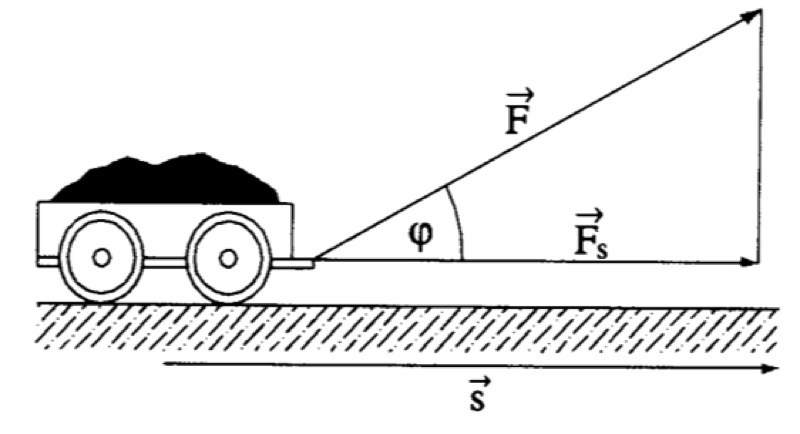
\includegraphics[width=0.49\textwidth]{pictures/arbeit}
\end{center}
\caption{Arbeit ist \glqq Kraft mal Weg\grqq}
\end{figure}

Benutzt man $F_s = F\cdot\cos\varphi$, so erhält man für die Arbeit
$$W = \V{F_s}\cdot\V{s} = F\cdot s \cdot \cos \varphi$$
Merkwürdig ist, dass die Verknüpfung zweier vektorieller Grässen (Kraft, Weg) eine skalare Grösse (Arbeit) ergibt. Ferner bemerken wir, dass die Länge von $\V{F_s}$ vom Winkel $\varphi$ abhängt.

\section{Zerlegung eines Vektors}
Die Zerlegung eines beliebigen Ortsvektors nach den Basisvektoren $\ex$ und $\ey$ im rechtwinkligen Koordinatensystem ist ein Spezialfall eines allgemeineren Sachverhalts. Insbesondere bei physikalischen Problemen muss man oft eine Kraft in zwei Teilkräfte, deren Richtungen vorgegeben sind, zerlegen.

\begin{bsps}
\ \\[-4ex]
\begin{itemize}
\item Die Lampe einer Strassenbeleuchtung hängt an zwei Spannseilen. Die Gewichtskraft der Lampe wird in zwei Teilkräfte mit vorgeschriebenen Richtungen zerlegt.
\item Eine Kugel mit der Gewichtskraft $\V{F_G}$ bindet sich auf einer schiefen Ebene mit Neigungswinkel $\ga$. $\V{F_G}$ lässt sich in die beiden Teilkräfte Hangabtriebskraft $\V{F_H}$ und Normalkraft $\V{F_N}$ zerlegen.
\end{itemize}
\end{bsps}

\begin{ueb}[Keil erforderlich?]
Eine $\unit[120]{m}$ lange Strasse steigt um $\unit[18]{m}$ an; auf ihr steht ein $\unit[42]{kN}$ schwerer Lastzug. Welche Kraft ist erforderlich, um ein Abwärtsrollen zu verhindern?
\end{ueb}
\section{Realistische Darstellungen mit dem Computer}
Wer kennt sie nicht, die Computergraphiken und -animationen in den Videoclips, in der Werbung, in kommerziellen und wissenschaftlichen Filmen, \dots?

\begin{itemize}
\item In einem Werbespot der Firma General Motors wird ein Sportwagen vom Typ Pontiac Fiero Bauteil für Bauteil über den Wolken montiert.
\item Für das Weltraum-Epos \glqq The Last Starfighter\grqq\ wurden im Computer --- ohne Modelle oder Zeichentrick-Vorlagen --- 27 Minuten Schlachtgetümmel und Sternreisen komponiert.
\item Die Digital Effects Studios in New York bauten im Computer einen Strassenzug Manhattans der 30er Jahre nach, in dem der Betrachter mit naturgetreu wechselnden Perspektiven zwischen Wolkenkratzern wandeln kann.
\item Am MIT wurde ein Computer-Trickfilm entwickelt, in dem ein nahezu lichtschnelles Raumschiff den Studenten die Tücken relativistischer Raumfahrt demonstriert.
\end{itemize}

Um wirklichkeitsgetreue Abbildungen zu erhalten, muss man die verschiedensten Dinge beachten wie zum Beispiel die Richtung des einfallenden Lichts, die Ober\-flä\-chen\-be\-schaf\-fen\-heit der darzustellenden Körper, deren Licht\-durch\-läs\-sig\-keit etc. In Wirklichkeit sind sehr wenige Flächen einfarbig. Oft beeinflussen Schattierungen, Spiegelbilder und durchscheinende Bilder das Ergebnis. Mit einfachen und komplizierten Algorithmen kann man heute schon sehr realistische Bilder erstellen. Im folgenden Abschnitt wird gezeigt, wie eine Tiefenwirkung durch die verschiedenen Be\-gren\-zungs\-flächen eines Körpers mit einer einfachen Idee erzeugt werden kann.

\begin{figure}
\begin{center}
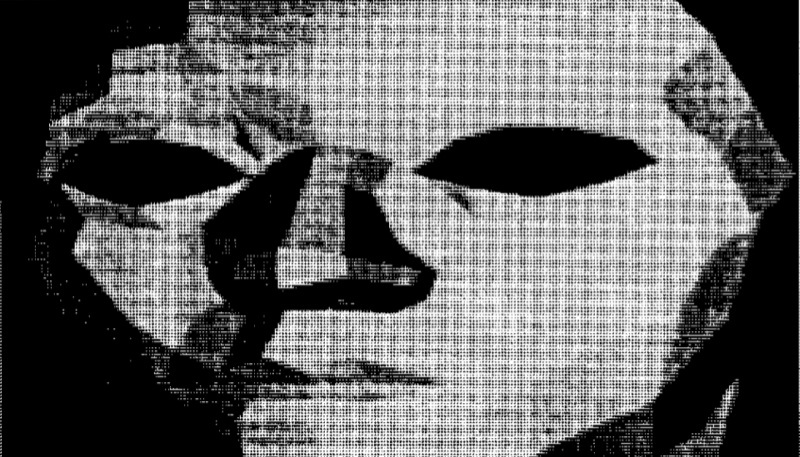
\includegraphics[width=0.7\textwidth]{pictures/pcgrafik}
\end{center}
\caption{Polygonmodell eines Kopfs}
\end{figure}

Wir gehen davon aus, dass der darzustellende Körper von einer Lichtquelle, die sich der Einfachheit halber im Unendlichen befindet, beleuchtet wird. Die Lichtstrahlen treffen auf die verschiedenen Begrenzungsflächen des Körpers auf und werden nach dem Reflexionsgesetz (Einfallswinkel=Ausfallswinkel) reflektiert.

\begin{figure}
\begin{center}
\definecolor{qqwuqq}{rgb}{0,0.39,0}
\definecolor{zzttqq}{rgb}{0.6,0.2,0}
\scalebox{0.8}{
\begin{tikzpicture}[line cap=round,line join=round,>=triangle 45,x=0.8cm,y=1.0cm]
\clip(-4.3,-0.72) rectangle (4.28,6.3);
\fill[color=zzttqq,fill=zzttqq,fill opacity=0.1] (-3.96,4.32) -- (-3,5) -- (0.72,-0.02) -- (-0.68,0) -- cycle;
\draw [shift={(-1.28,2.68)},color=qqwuqq,fill=qqwuqq,fill opacity=0.05] (0,0) -- (35.2:2) arc (35.2:51.25:2) -- cycle;
\draw [shift={(-1.28,2.68)},color=qqwuqq,fill=qqwuqq,fill opacity=0.05] (0,0) -- (20.87:2) arc (20.87:35.2:2) -- cycle;
\draw [color=zzttqq] (-3.96,4.32)-- (-3,5);
\draw [color=zzttqq] (-3,5)-- (0.72,-0.02);
\draw [color=zzttqq] (0.72,-0.02)-- (-0.68,0);
\draw (-1.28,2.68)-- (2.86,5.6);
\draw (-1.28,2.68)-- (1.4,6.02);
\draw (-1.28,2.68)-- (3.18,4.38);
\draw [->] (1.4,6.02) -- (0.02,4.3);
\draw [->] (-1.28,2.68) -- (0.8,3.47);
\draw[color=qqwuqq] (0,3.8) node {$\varphi$};
\draw[color=qqwuqq] (0.3,3.5) node {$\varphi$};
\end{tikzpicture}
}
\end{center}
\caption{Lichtreflexion an glatter Oberfläche}
\end{figure}

Man nimmt nun an, dass die Helligkeit einer Fläche nur durch den Einfallswinkel $\varphi$ bestimmt wird. In der Informatik benutzt man die \emph{Lambert'sche Regel}, die besagt, dass der Anteil des jeweils reflektierten Lichts gleich dem Cosinus des Einfallswinkels $\varphi$ ist.
Wenn $L$ die Intensität der Lichtquelle ist, so berechnet sich die Helligkeit $H$ der darzustellenden Fläche durch
$$H(\varphi)=k\cdot L\cdot\cos(\varphi)$$
wobei $k$ eine Materialkonstante ist. $k$ nimmt Werte zwischen $0$ und $1$ an und gibt den Prozentsatz des reflektierten Lichts an.

Mit Hilfe dieser einfachen Methode kann man mit verhältnismässig wenig Rechenaufwand schon erstaunlich gute Bilder erstellen.

\begin{ueb}[Lambert]
Der abgebildete Würfel wird aus der Richtung
$$\vv=\pV{-3}{-2}{-1}$$
bestrahlt. Berechne für $k=0.5$ und $L=1$ die Helligkeiten, mit der die drei beleuchteten Würfelflächen eingefärbt werden sollen. Färbe die drei Flächen mit drei verschiedenen Grautönen ein.
\begin{center}
\scalebox{0.8}{
\begin{tikzpicture}[line cap=round,line join=round,>=triangle 45,x=0.8cm,y=0.8cm]
\clip(-4.3,-0.76) rectangle (6.12,6.3);
\draw [->,dash pattern=on 2pt off 2pt] (-3,1) -- (4.5,1);
\draw [->,dash pattern=on 2pt off 2pt] (-1,0) -- (-1,6);
\draw [->,dash pattern=on 2pt off 2pt] (0.3,1.66) -- (-4.06,-0.54);
\draw (-3,0)-- (1,0);
\draw (1,0)-- (3,1);
\draw (-3,0)-- (-3,4);
\draw (1,0)-- (1,4);
\draw (3,1)-- (3,5);
\draw (-3,4)-- (-1,5);
\draw (-3,4)-- (1,4);
\draw (1,4)-- (3,5);
\draw (-1,5)-- (3,5);
\draw (-3,0)-- (-1,1);
\draw (-1,1)-- (-1,5);
\draw (-1,1)-- (3,1);
\draw (-3.7,0.5) node[anchor=north west] {1};
\draw (3.2,1.6) node[anchor=north west] {1};
\draw (-1.5,5.7) node[anchor=north west] {1};
\end{tikzpicture}
}
\end{center}
\end{ueb}

\begin{figure}[ht]
\begin{center}
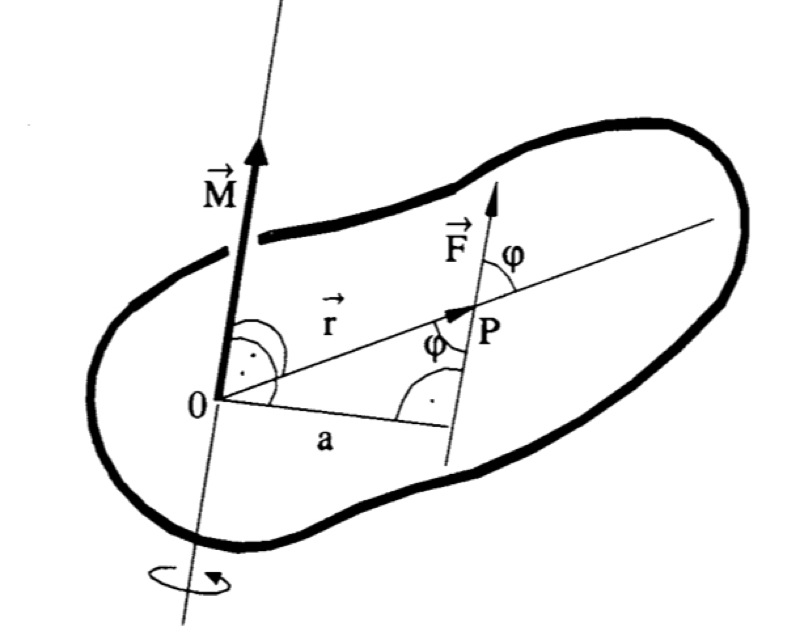
\includegraphics[width=5cm]{pictures/vprodukt}
\end{center}
\caption{Drehmoment $\V{M}$}\label{abb:vektorprod}
\end{figure}

Auf den Körper wirke im Punkt $P$ eine Kraft $\V{F}$ wie in Abbildung \ref{abb:vektorprod} auf Seite \pageref{abb:vektorprod} skizziert. Für die Berechnung des Drehmoments $M$ benötigt man nicht die Entfernung $r =\overline{OP}$, sondern den Abstand $a =r\cdot\sin\varphi$ der Wirkungslinie der Kraft vom Drehpunkt $O$:
$$M =a\cdot F =r\cdot F\cdot \sin\varphi$$

Physikalische Experimente zeigen:
\begin{itemize}
\item die Drehachse steht senkrecht zur Ebene, die durch
$\V{r}$ und $\V{F}$ aufgespannt wird,
\item die Drehrichtung wird durch $\V{r}$ und $\V{F}$ so bestimmt,
dass ein rechtshändiges System vorliegt ($\V{r}$: Daumen,
$\V{F}$: Zeigefinger, Drehrichtung: Mittelfinger der rechten Hand).
\end{itemize}
Man schreibt dafür:
$$\V{M}=\V{r}\times\V{F}$$
(lies: \glqq $r$ Kreuz $F$\grqq)

\begin{bsp}
Eine nützliche Anwendung zeigt sich in der Elektrotechnik zur Bestimmung der Richtung der Lorentzkraft. Es gilt nämlich
$$\vec{F}=Q\cdot(\vv\times\vec{B}),$$
wobei $Q$ für die Ladung, $\vv$ für die Geschwindigkeit der Ladung und $\vec{B}$ für das Magnetfeld steht.
\begin{figure}
\begin{center}
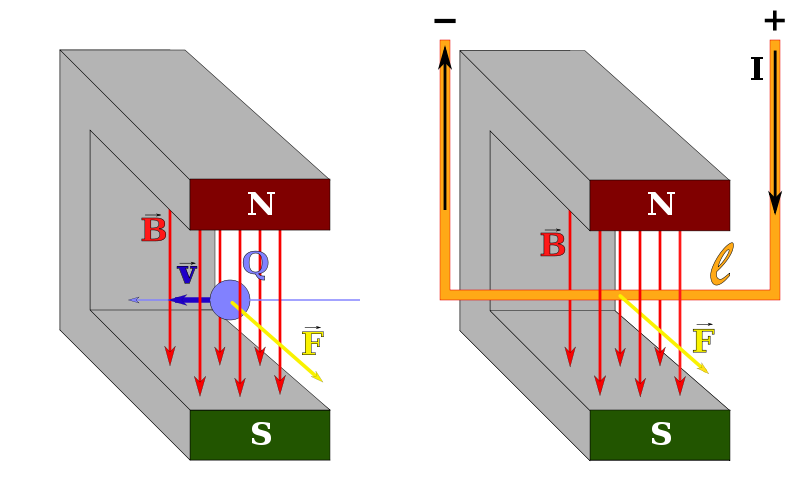
\includegraphics[width=0.4\textwidth]{pictures/lorentz.png}
\caption{Lorentzkraft $\vec{F}$}
\end{center}
\end{figure}
Der ausgestreckte rechte Zeigefinger folgt der technischen Stromrichtung, also der Bewegungsrichtung von positiv geladenen Ladungsträgern bzw. der entgegengesetzten Bewegungsrichtung negativer Ladungsträger.
Der ausgestreckte rechte Mittelfinger folgt der Richtung der Magnetfeldlinien, also der Richtung, in die sich der Nordpol eines Probemagneten ausrichtet.
Der rechte Daumen zeigt nun in die Wirkungsrichtung der Lorentzkraft.
\end{bsp}

\cleardoublepage

\listoffigures

\end{document}